El diseño de la interfaz ha sido basado en la implementación de los requisitos del sistema que han sido definidos en el apartado \ref{req.fun}.

En cuanto a la interfaz de usuario, se ha buscado seguir los patrones de \textit{responsive web design}, permitiendo la adaptación del contenido de la página en función del dispositivo el cual la esté cargando, pudiendo ser tanto monitores de ordenadores, como tablets o smartphones.

\begin{enumerate}

    \item \textbf{Dashboard} %%% DASHBOARD
    
Se prediseñó un panel de dashboard en el cual los dispositivos apareciesen como recuadros de colores, que cambiasen su color en función del estado.
Al pulsar un color, se abriría una tarjeta en la cual aparecería la información relativa al dispositivo.

    \begin{figure}[H]
        \centering
        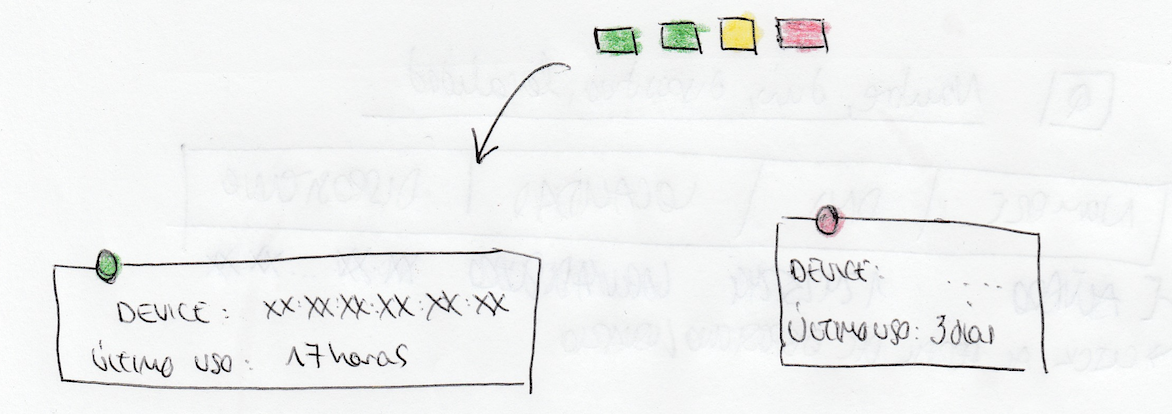
\includegraphics[width=10cm]{./img/web/devices/dev.pre.png}
        \caption{Dashboard: Planteamiento de diseño}
        \label{fig:devices.pre}
    \end{figure}

Finalmente, pese a  que esta opción permitía la visualización de cientos de dispositivos a la vez, no proporcionaba una buena identificación de qué recuadro era un dispositivo concreto, o cuánto tiempo exacto había pasado.
Por ello, se optó por mostrar directamente las tarjetas de los dispositivos, cambiando la forma en que aparecen los colores y haciéndola más fácil de comprender, localizar e identificar un dispositivo concreto.

En las siguientes figuras aparecen las posibles variaciones de las tarjetas.
    
    \begin{figure}[H]
        \centering
        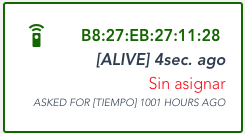
\includegraphics[width=4cm]{./img/web/devices/dev.green.png}
        \caption{Dashboard: Dispositivo en línea}
        \label{fig:web.dir}
    \end{figure}
    
    \begin{figure}[H]
        \centering
        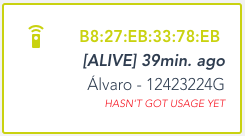
\includegraphics[width=4cm]{./img/web/devices/dev.greellow.png}
        \caption{Dashboard: Dispositivo reciente}
        \label{fig:web.dir}
    \end{figure}
    
    \begin{figure}[H]
        \centering
        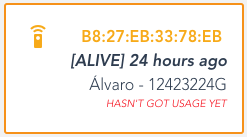
\includegraphics[width=4cm]{./img/web/devices/dev.orange.png}
        \caption{Dashboard: Dispositivo ausente}
        \label{fig:web.dir}
    \end{figure}
    
    \begin{figure}[H]
        \centering
        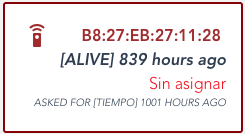
\includegraphics[width=4cm]{./img/web/devices/dev.red.png}
        \caption{Dashboard: Dispositivo posiblemente apagado}
        \label{fig:web.dir}
    \end{figure}
    
    \begin{figure}[H]
        \centering
        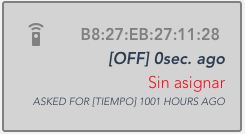
\includegraphics[width=4cm]{./img/web/devices/dev.grey.png}
        \caption{Dashboard: Dispositivo apagado por comando}
        \label{fig:web.dir}
    \end{figure}
    
    \begin{figure}[H]   
        \centering
        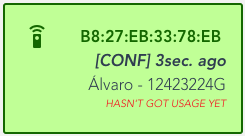
\includegraphics[width=4cm]{./img/web/devices/dev.doing.png}
        \caption{Dashboard: Dispositivo realizando tarea enviada}
        \label{fig:web.dir}
    \end{figure}
    
    En el dashboard, con el fin de poder localizar más rápidos los dispositivos que cumplan una serie de condiciones, se debe permitir un filtrado de ellos:
    \begin{enumerate}
        \item El dispositivo tiene un usuario asignado o no.
        \item Se ordenan por fecha de su última actividad, o por fecha de su última tarea.
        \item Ese orden es realizado de manera ascendente, o descendente.
    \end{enumerate}
    
    El panel que permitiese este filtrado fue prediseñado de manera simple en una ventana emergente que recibe el nombre de \textit{modal} en el mundo del desarrollo web, facilitando de manera simple y efectiva la realización, como se puede ver a continuación.
    
    \begin{figure}[H]   
        \centering
        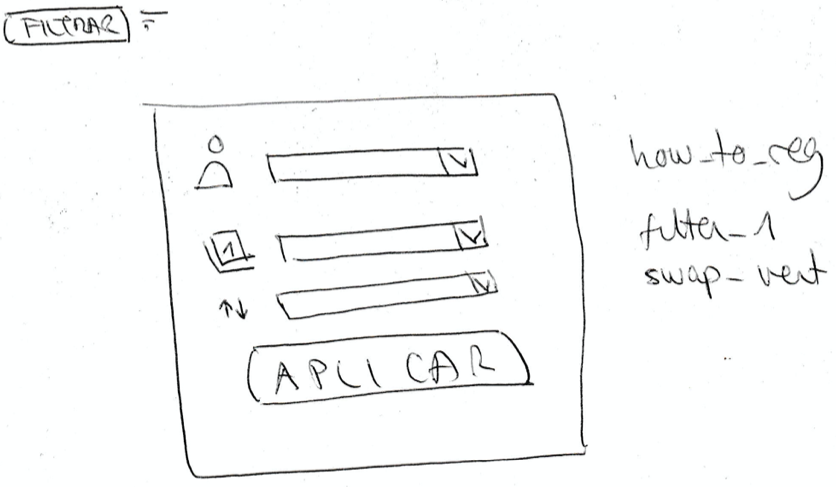
\includegraphics[width=7cm]{./img/web/devices/dev.filter.pre.png}
        \caption{Dashboard - Planteamiento del filtro de dispositivos}
        \label{fig:web.dir}
    \end{figure}
    
    El diseño final implementado no tuvo ningún cambio ya que el plantemiento del diseño cumplía con las expectativas, ofreciendo una satisfactoria experiencia de usuario.
    
    \begin{figure}[H]   
        \centering
        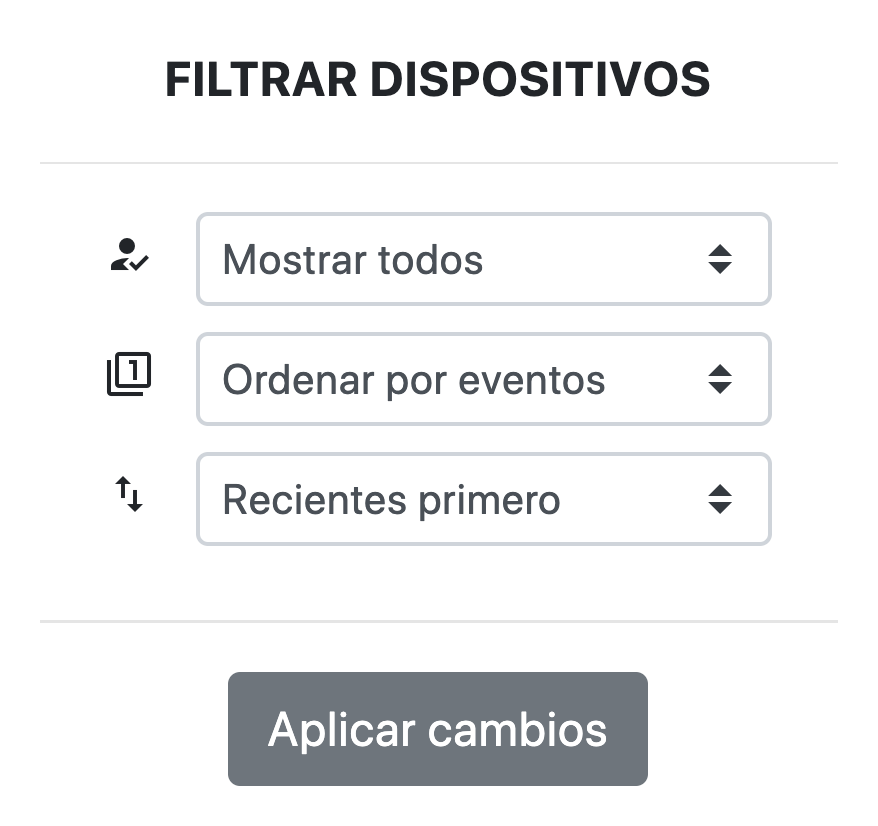
\includegraphics[width=8cm]{./img/web2/home.device.filter.png}
        \caption{Dashboard - Diseño final del filtro de dispositivos}
        \label{fig:web.dir}
    \end{figure}
    
    En cuanto a las tarjetas en las cuales aparece la información del dispositivo, deben permitir un acceso a la visualización de estadísticas, o a la selección rápida de tareas. También, debe permitir servir de punto base para acceder a otros servicios del sistema como puede ser la configuración de los parámetros del dispositivo.
    
    \begin{figure}[H]   
        \centering
        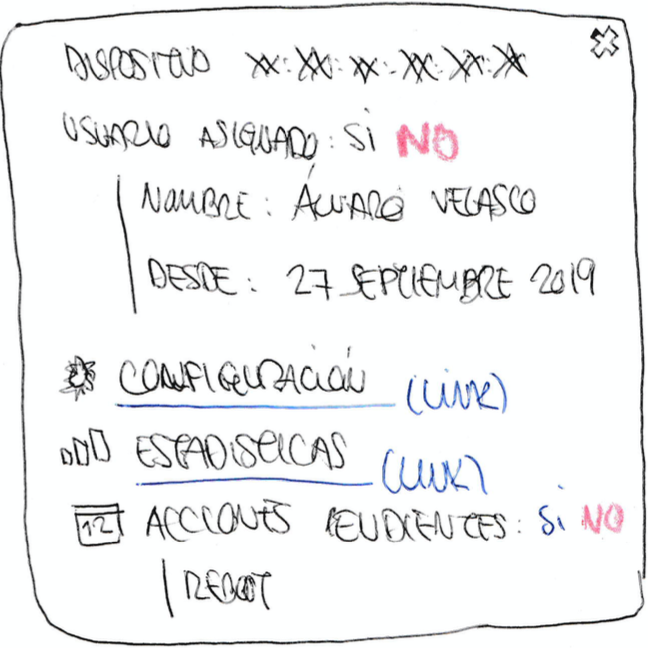
\includegraphics[width=7cm]{./img/web/devices/dev.quick.pre.png}
        \caption{Dashboard - Planteamiento de diseño de acciones rápidas.}
        \label{fig:web.dir}
    \end{figure}    
    
    \begin{figure}[H]   
        \centering
        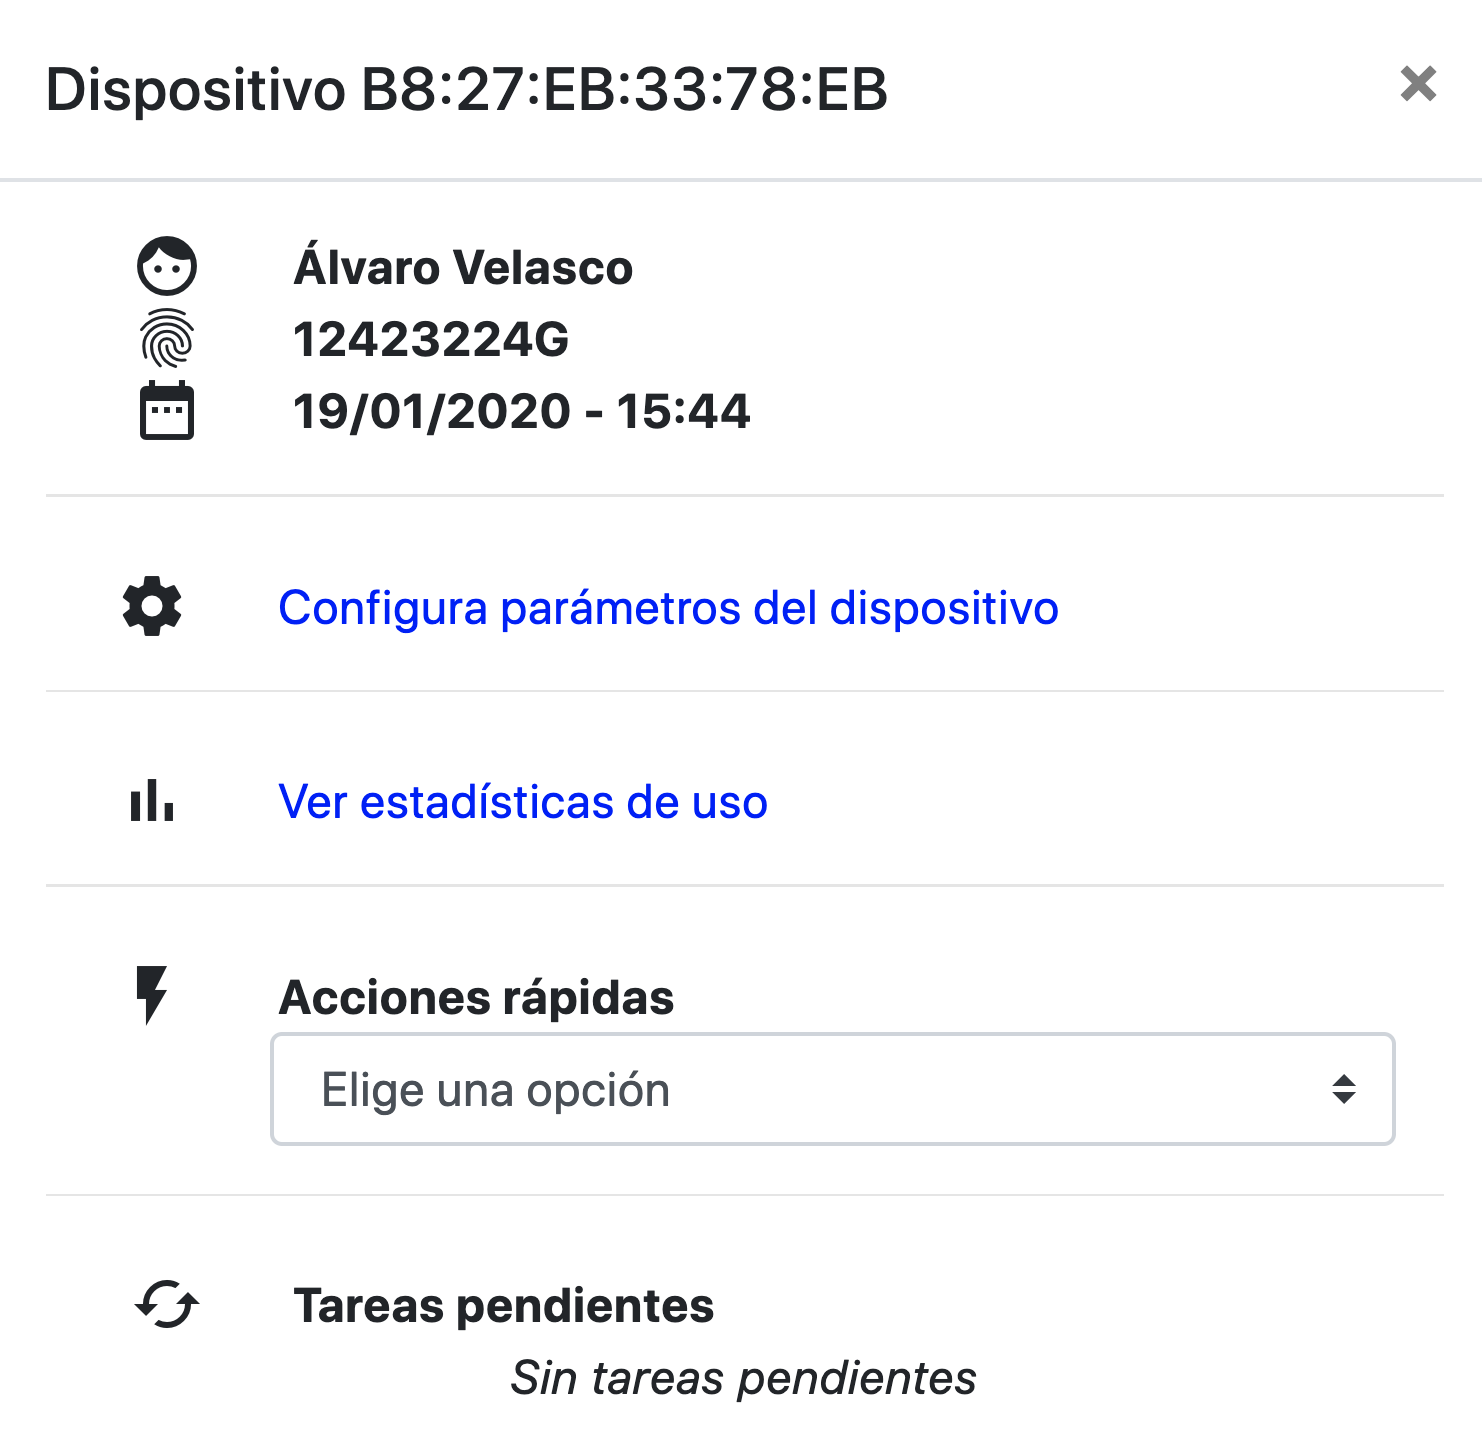
\includegraphics[width=9cm]{./img/web2/home.device.info.user}
        \caption{Dashboard - Diseño final de acciones rápidas: dispositivo asignado.}
        \label{fig:web.dir}
    \end{figure}
    
    \begin{figure}[H]   
        \centering
        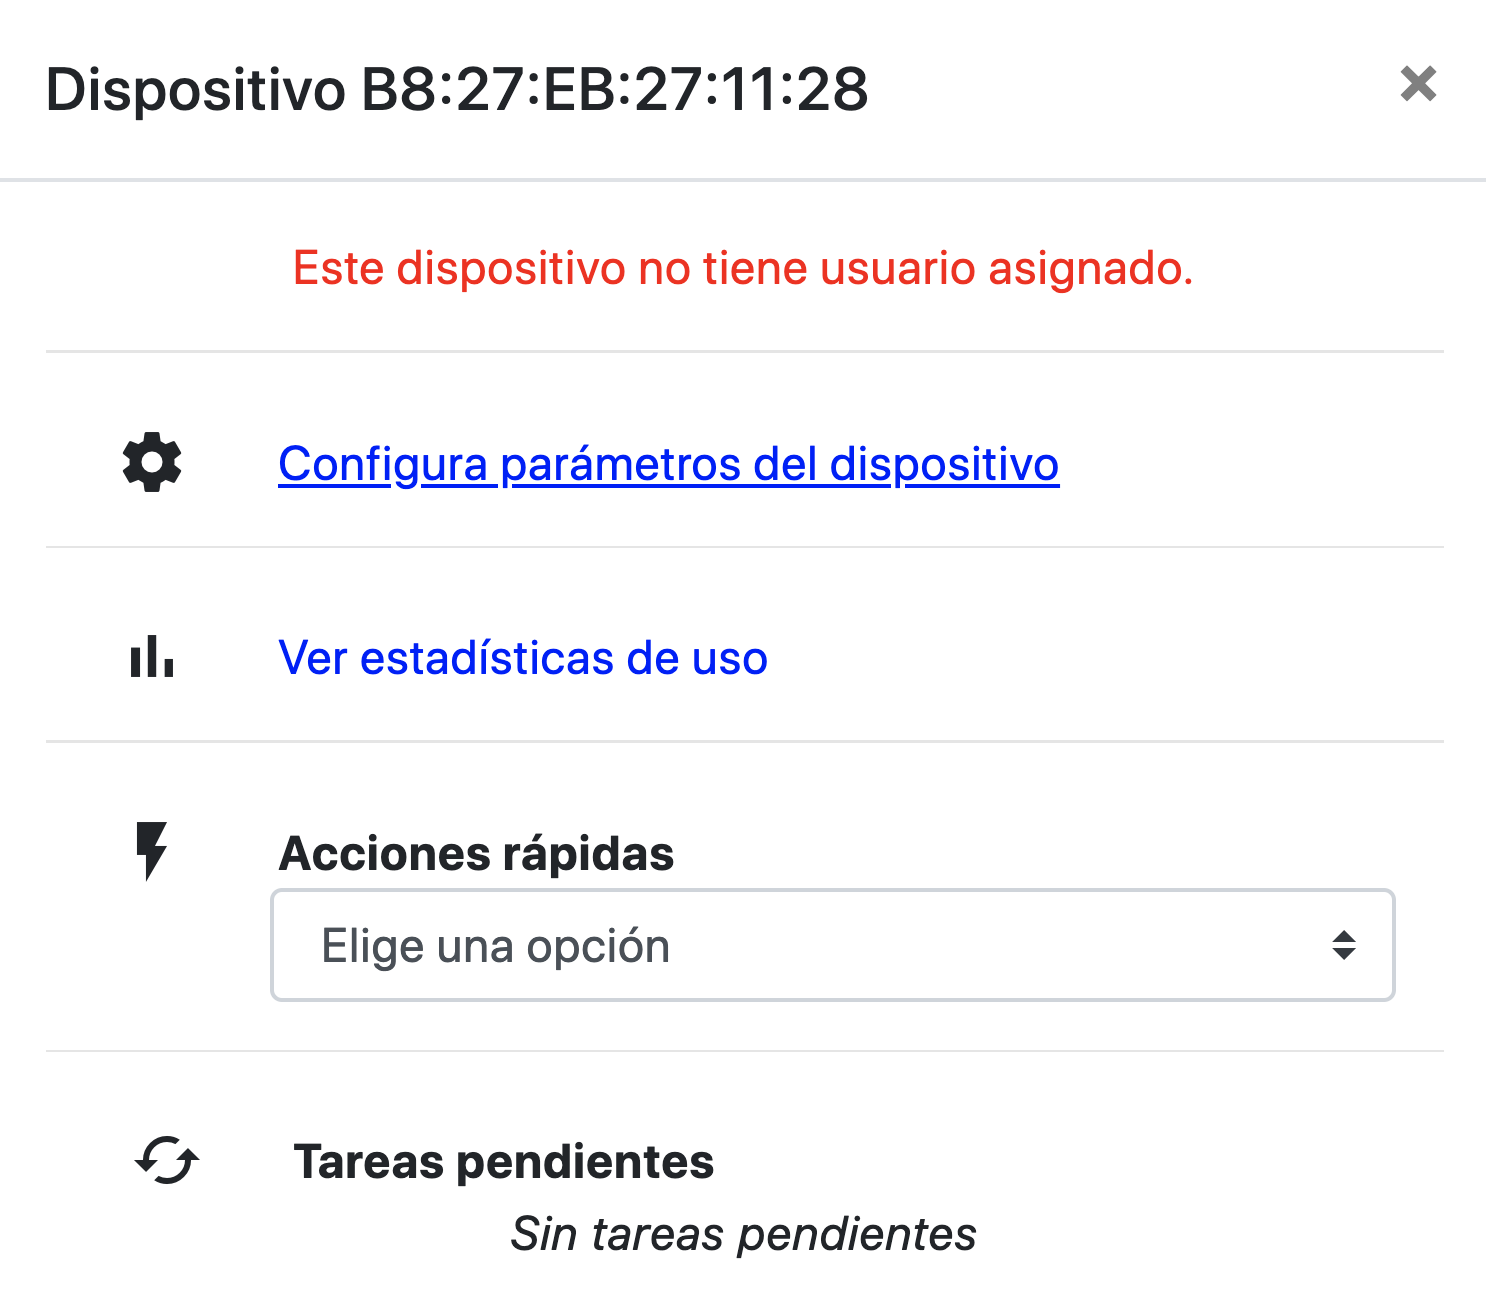
\includegraphics[width=9cm]{./img/web2/home.device.info}
        \caption{Dashboard - Diseño final de acciones rápidas: dispositivo sin asignar.}
        \label{fig:web.dir}
    \end{figure}
    
    
    \item \textbf{Localidades} %%% LOCALIDADES
    
    En esta sección se buscaba la posibilidad de ver una lista detallada de qué localidades estaban registradas en el sistema, al igual que cuántos dispositivos o personas estaban asocidados a cada localidad.
    
    Se contempló como buena idea en los diseños previos la posibilidad de una lista de provincias que contengan alguna localidad registrada mostrando las estadisticas generales, y que pulsando en ellas, se abriese la lista de localidades asociadas, con sus datos particulares.
    
    \begin{figure}[H]   
        \centering
        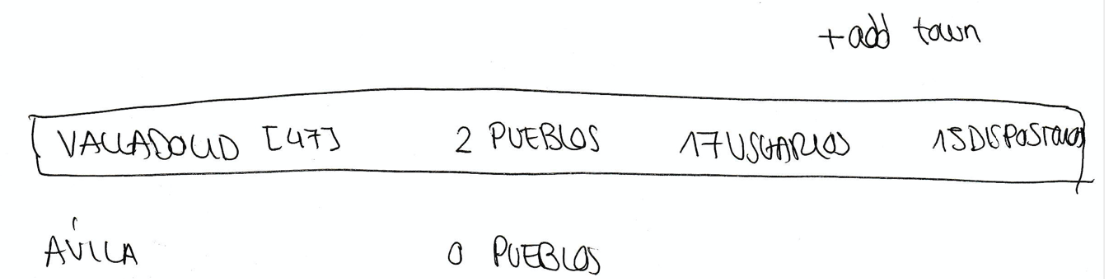
\includegraphics[width=11cm]{./img/web/locations/locations.closed.pre.png}
        \caption{Localidades - Planteamiento de lista: agrupado por provincias.}
        \label{fig:web.dir}
    \end{figure}
    
    \begin{figure}[H]   
        \centering
        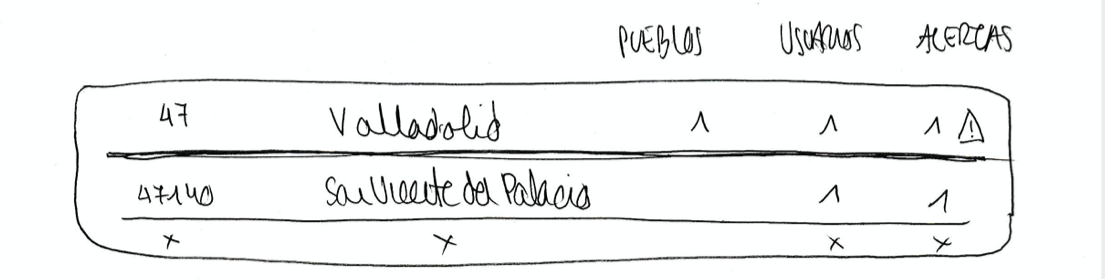
\includegraphics[width=11cm]{./img/web/locations/locations.opened.pre.png}
        \caption{Localidades - Planteamiento de lista: despliegue de provincia.}
        \label{fig:web.dir}
    \end{figure}
    
    \begin{figure}[H]   
        \centering
        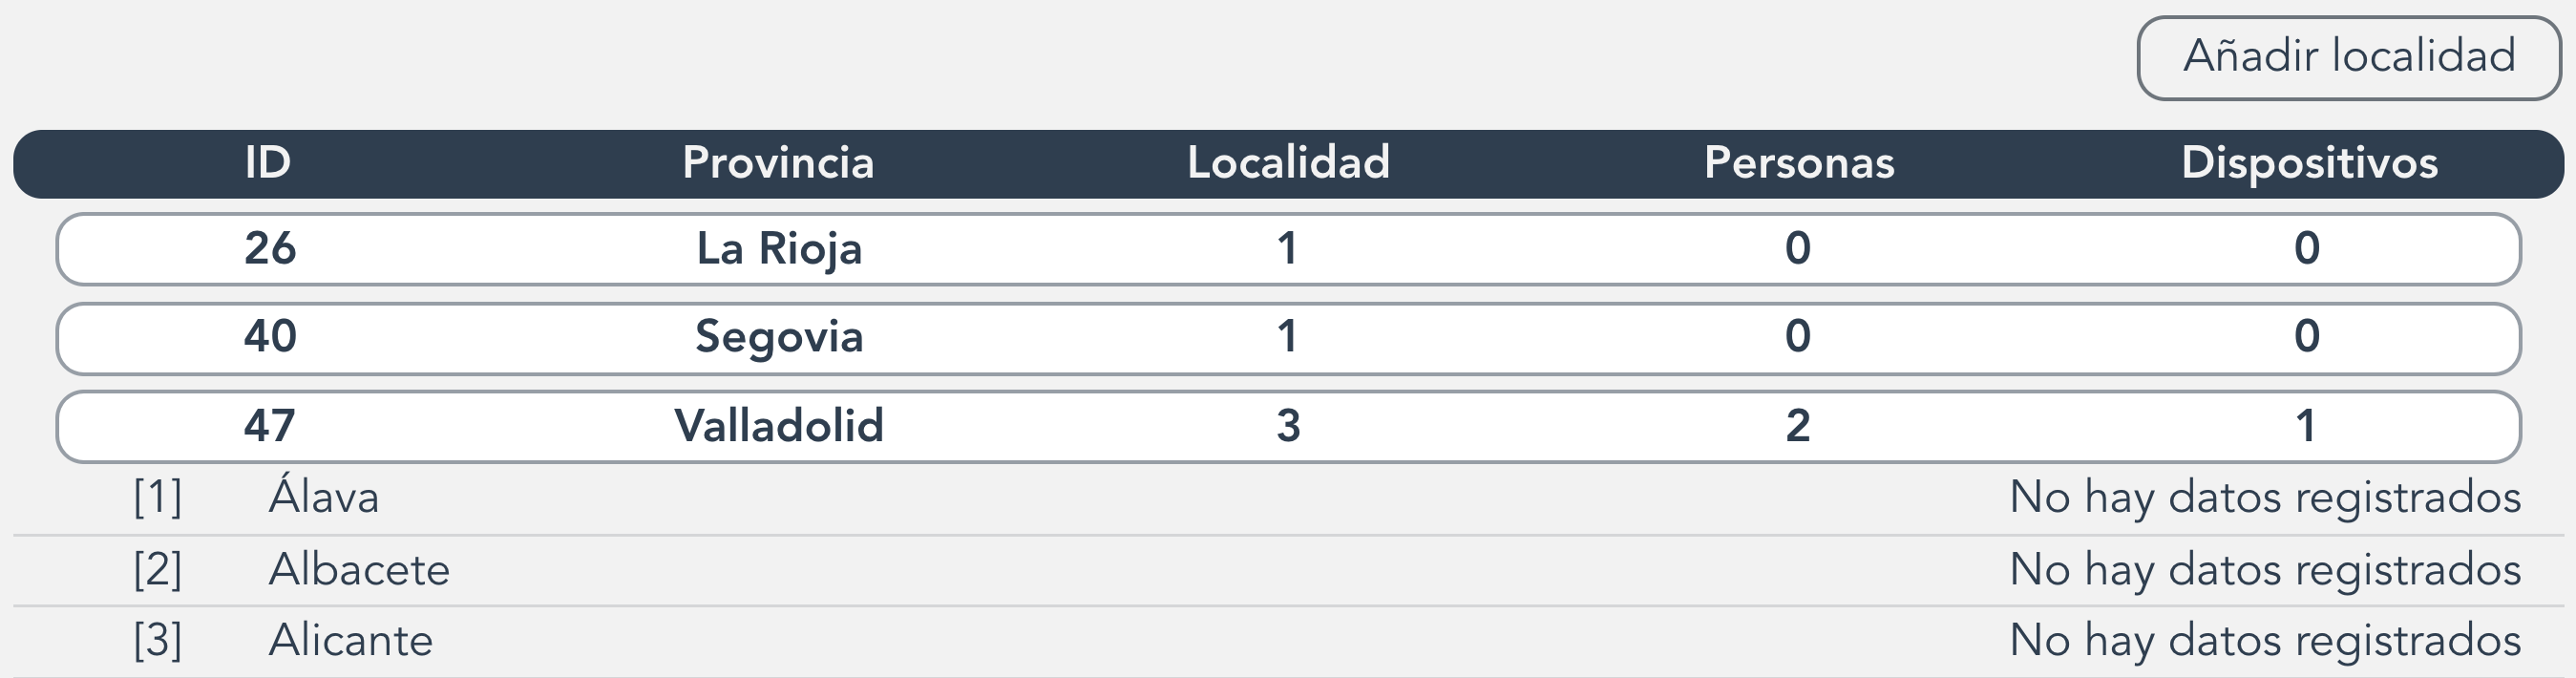
\includegraphics[width=11cm]{./img/web2/locations.table.png}
        \caption{Localidades - Diseño final de lista: agrupado por provincias.}
        \label{fig:web.dir}
    \end{figure}
    
    \begin{figure}[H]   
        \centering
        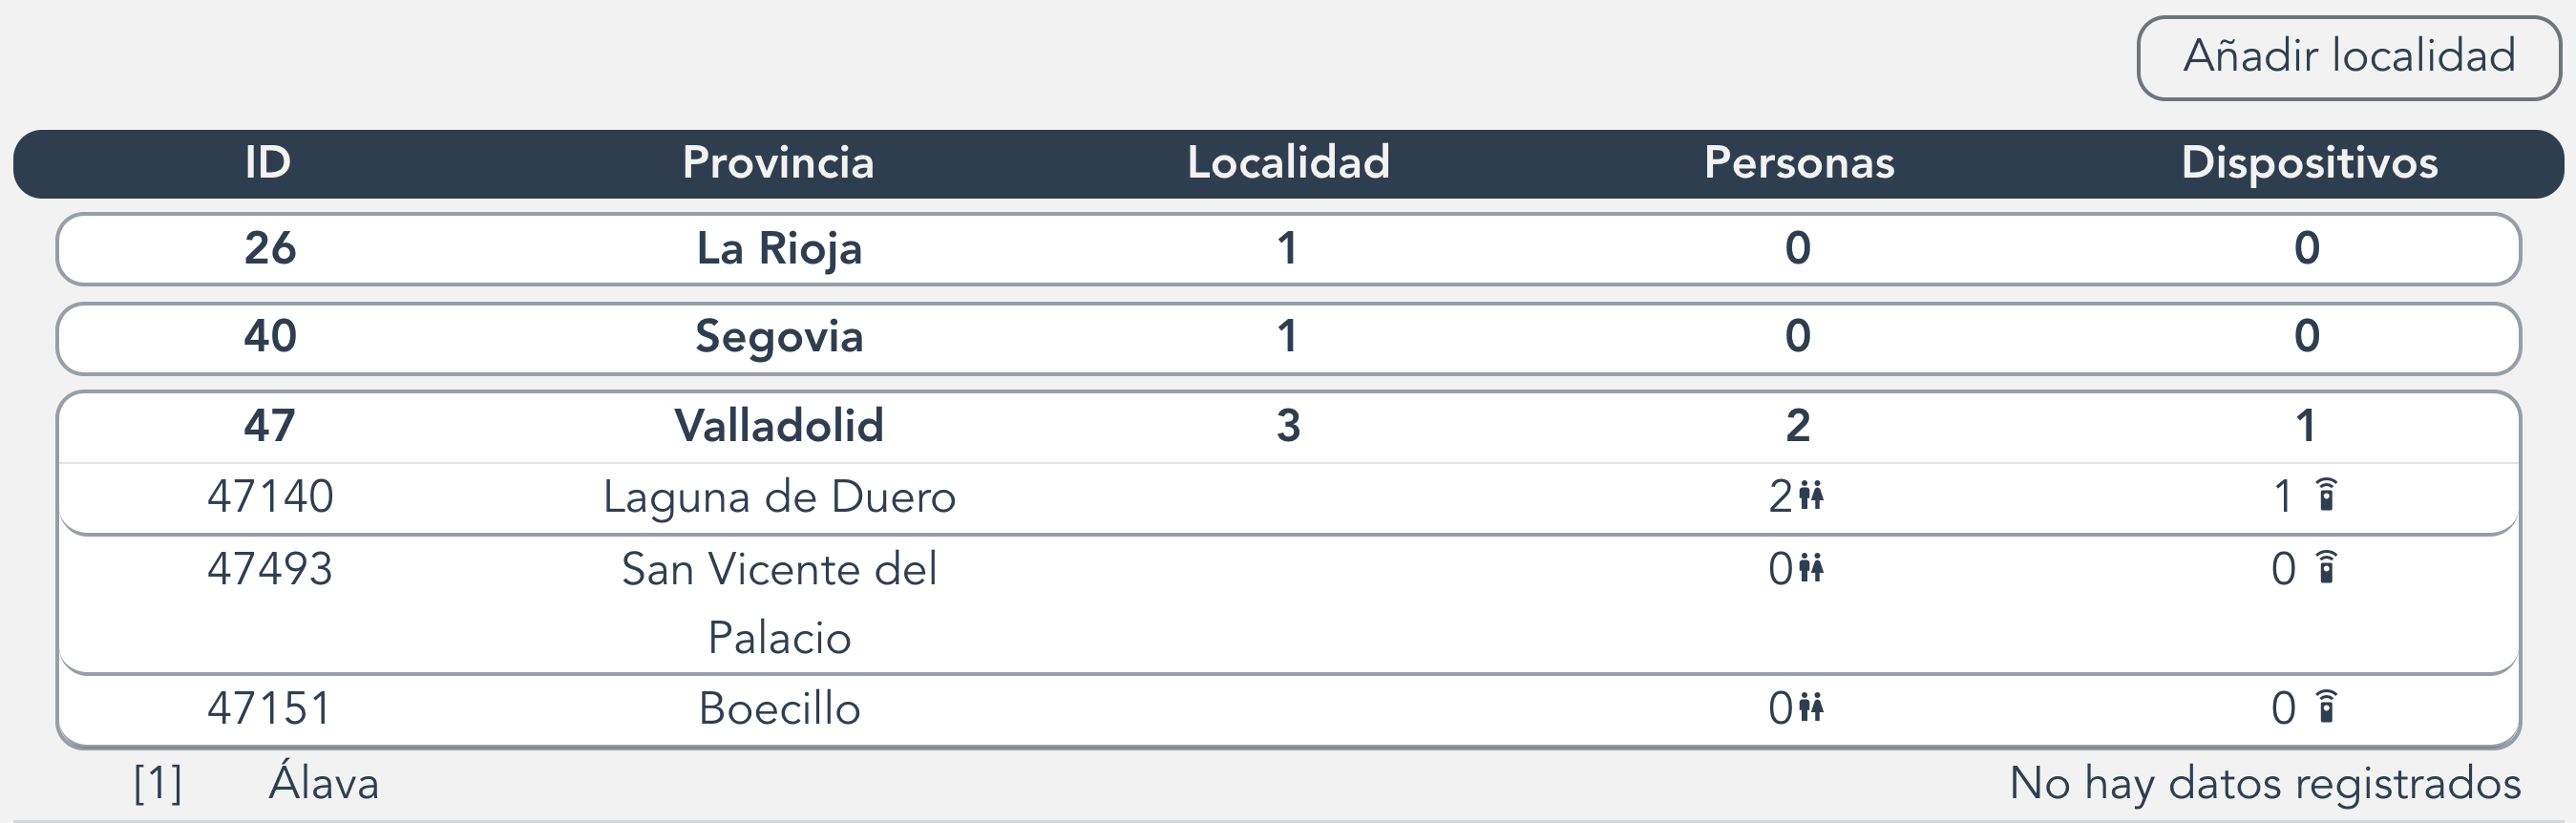
\includegraphics[width=11cm]{./img/web2/locations.table.opened.png}
        \caption{Localidades - Diseño final de lista: despliegue de provincia.}
        \label{fig:web.dir}
    \end{figure}
    
    En cuanto al diseño final se puede apreciar la posibilidad de añadir nuevas localidades. Para ello se planteó la posibilidad de añadirlo vía formulario: nombre de la localidad, código postal, provincia, y posición geográfica.
    
    \begin{figure}[H]   
        \centering
        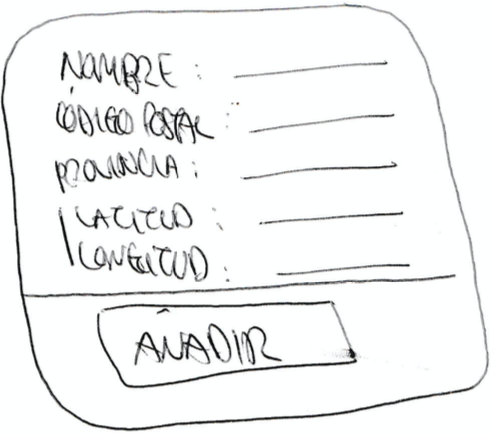
\includegraphics[width=6cm]{./img/web/locations/locations.add.pre.png}
        \caption{Localidades - Planteamiento de diseño para añadir nueva localidad.}
        \label{fig:location.add.post}
    \end{figure}
    
    Este prediseño, se ve que no es muy útil ya que la posición geográfica tendríamos que buscarla en otros servicios de mapas, o por que se debería introducir demasiados datos. 
    
    Finalmente se rediseñó, cambiando este prediseño por la implementación de un mapa que permitiese la búsqueda de la localidad, y añadirla seleccionándola en el mapa, de tal manera que se guarden todos los datos del formulario automáticamente sin necesidad de rellenarlos a mano, mejorando la experiencia de usuario.
    
    \begin{figure}[H]   
        \centering
        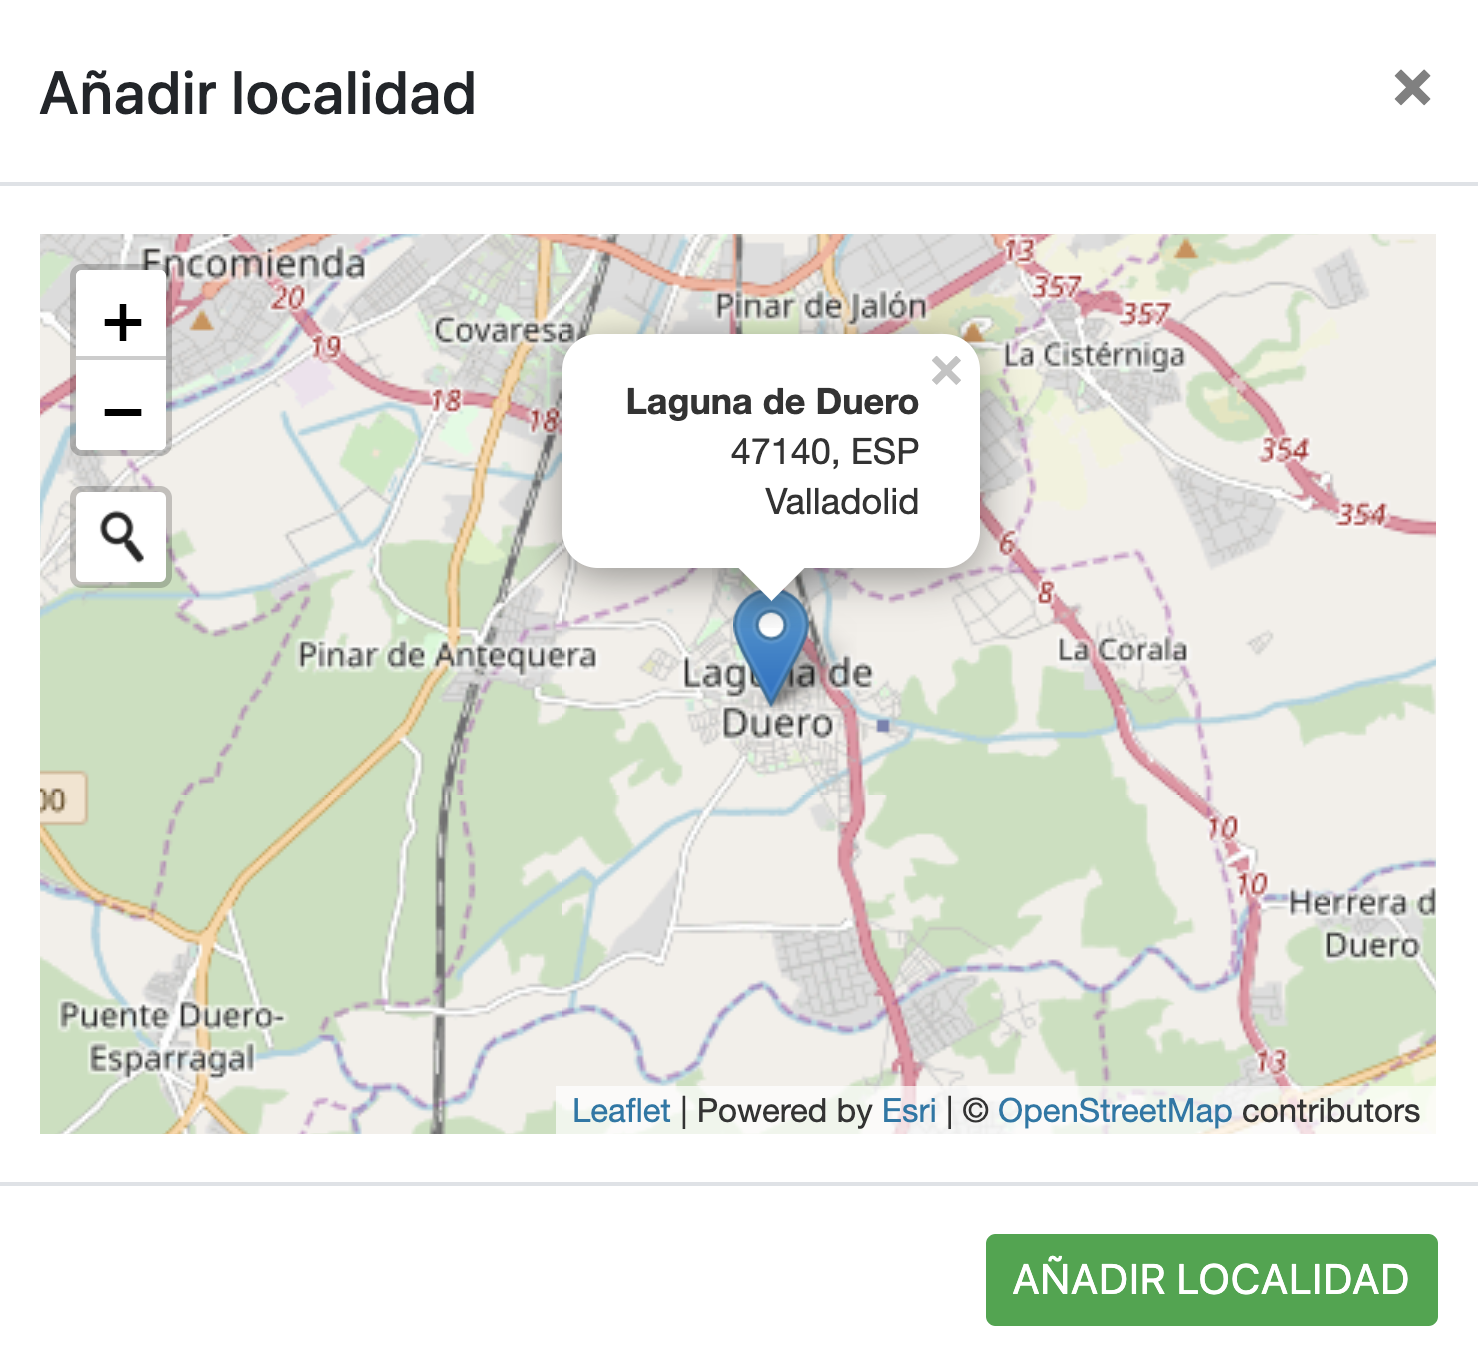
\includegraphics[width=8cm]{./img/web2/locations.add.map.png}
        \caption{Localidades - Diseño final de añadir nueva localidad.}
        \label{fig:location.add.post}
    \end{figure}
    
    En cuanto a la lista de localidades desplegada, un click sobre una localidad específica nos debería llevar al panel de configuraciones, permitiendo cambiar también la configuración de esa localidad.
    
    \item \textbf{Settings} %%% SETTINGS
    
    En esta sección se permite cambiar las configuracion prestablecida global. En caso de que se acceda a través de un enlace de una localidad, se permitirá cambiar la configuración de esa localidad, y en caso de acceder desde un dispositivo, se permitirá cambiar tango la global, como la del dispositivo, como la del pueblo del usuario asignado, en caso de que lo tenga.
    
    \begin{figure}[H]   
        \centering
        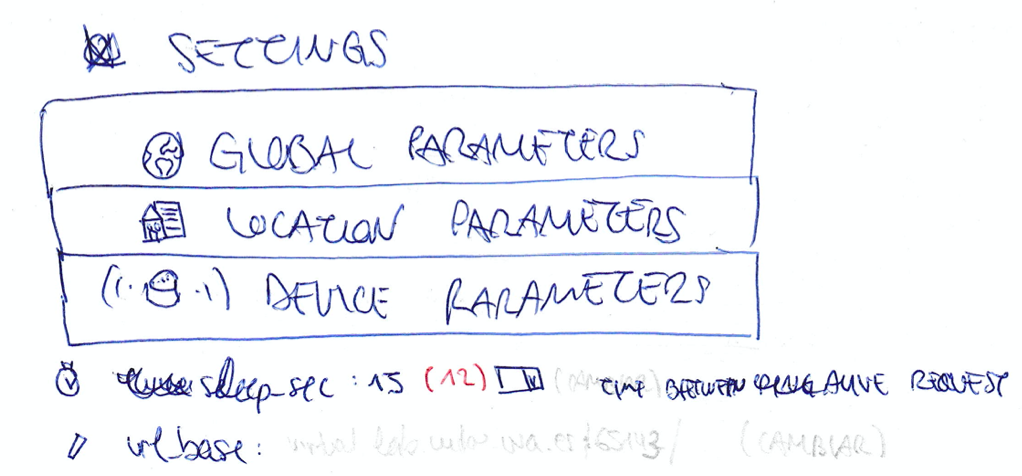
\includegraphics[width=10cm]{./img/web/settings/settings.pre.png}
        \caption{Settings - Planteamiento de diseño de configuraciones.}
        \label{fig:set.pre}
    \end{figure}
    
    De este planteamiento de diseño se han podido sacar aspectos interesantes, como la posibilidad de mostrar la configuración específica de un dispositivo, o si tiene aún alguna configuración pendiente específica por instalar mostrando esos valores pendientes en rojo al lado del valor que tiene instalado.
    
    En cuanto a la implementación real, se muestra cómo solo se ha definido al configuración de tiempo entre avisos, pudiendo ser esta parametrización fácilmente ampliable añadiendo simplemente nuevos campos, ya que la base y la lógica ya está montada.
    
    \begin{figure}[H]   
        \centering
        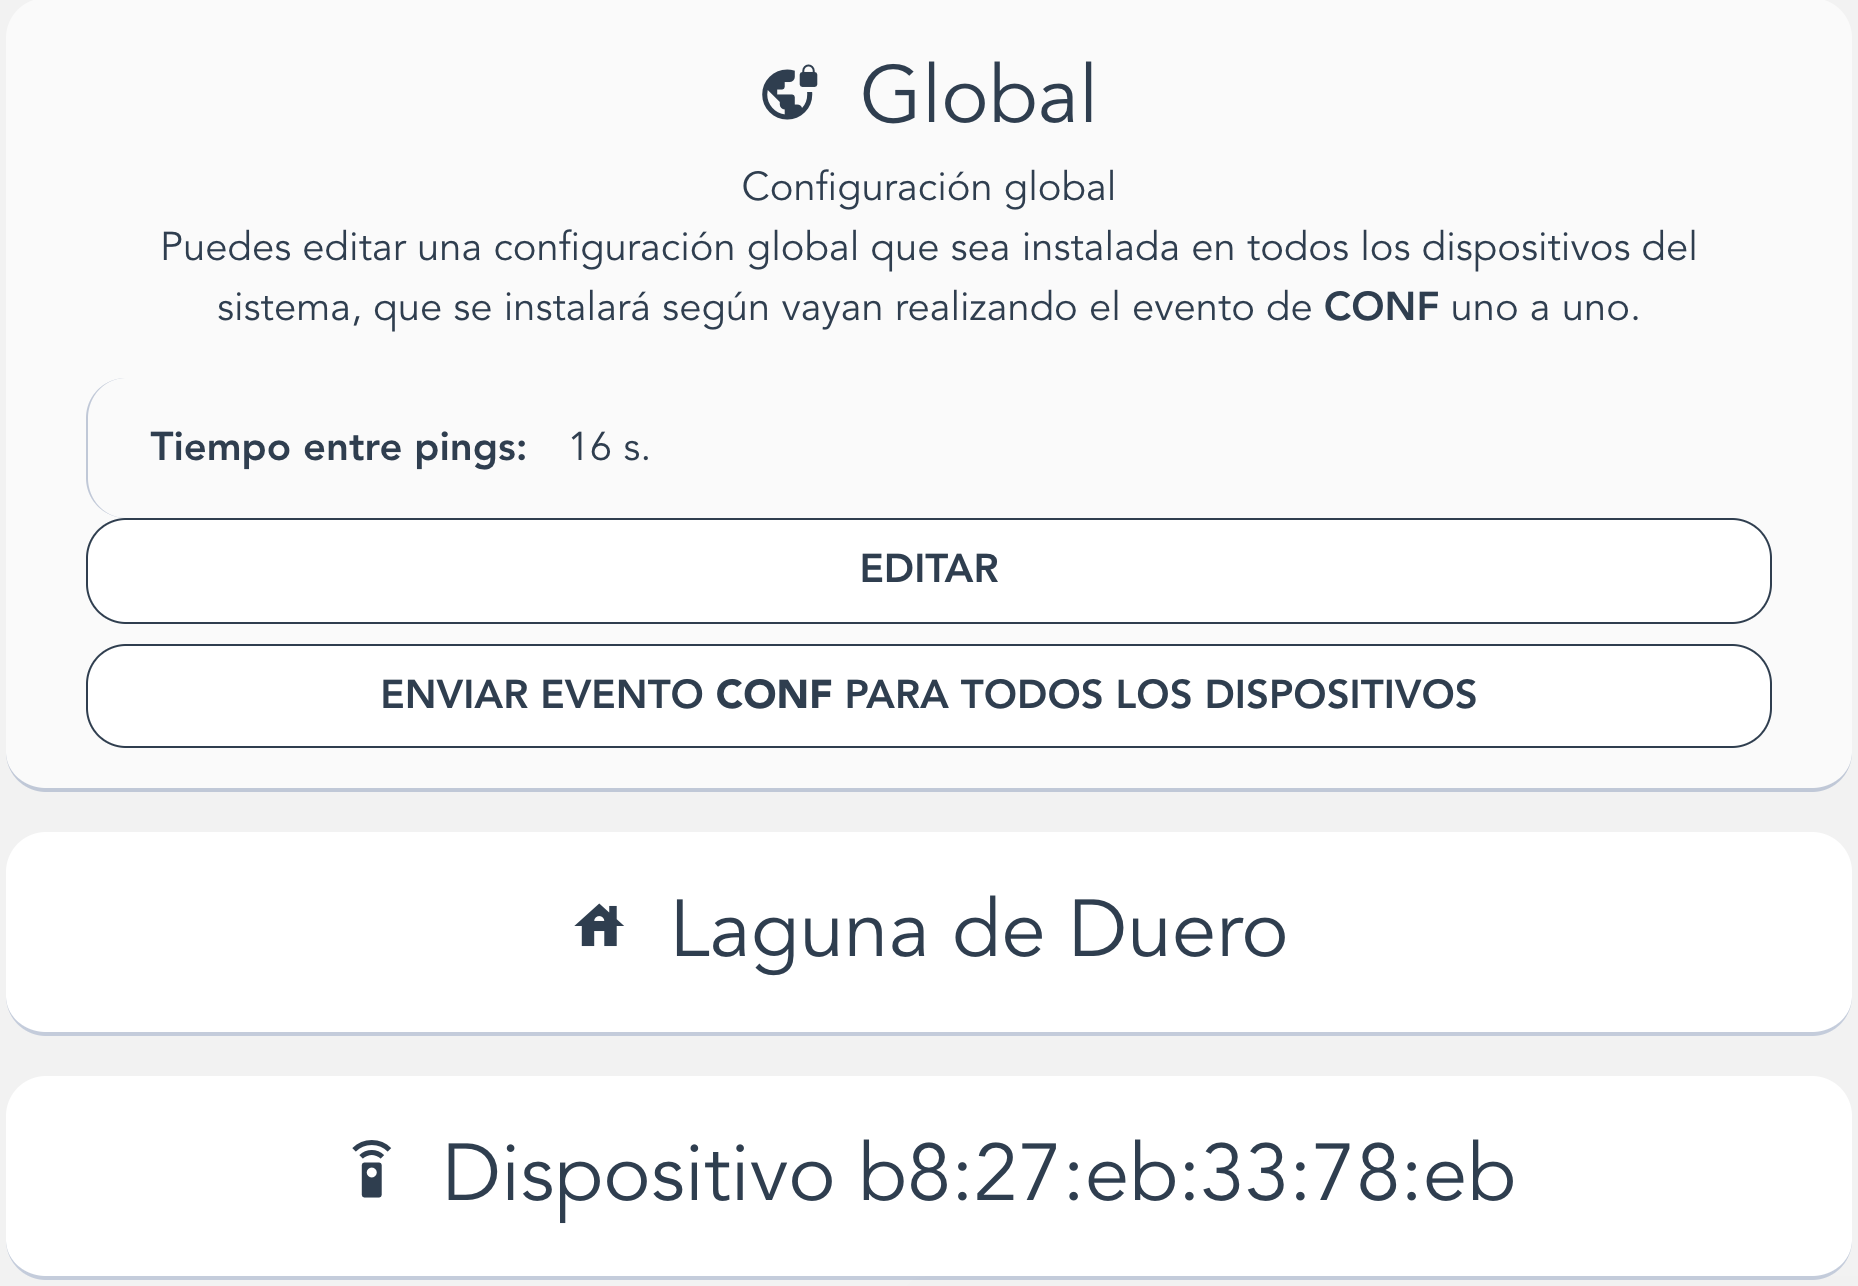
\includegraphics[width=10cm]{./img/web2/settings.global.png}
        \caption{Settings - Diseño final de configuración global.}
        \label{fig:set.global}
    \end{figure}
    
    \begin{figure}[H]   
        \centering
        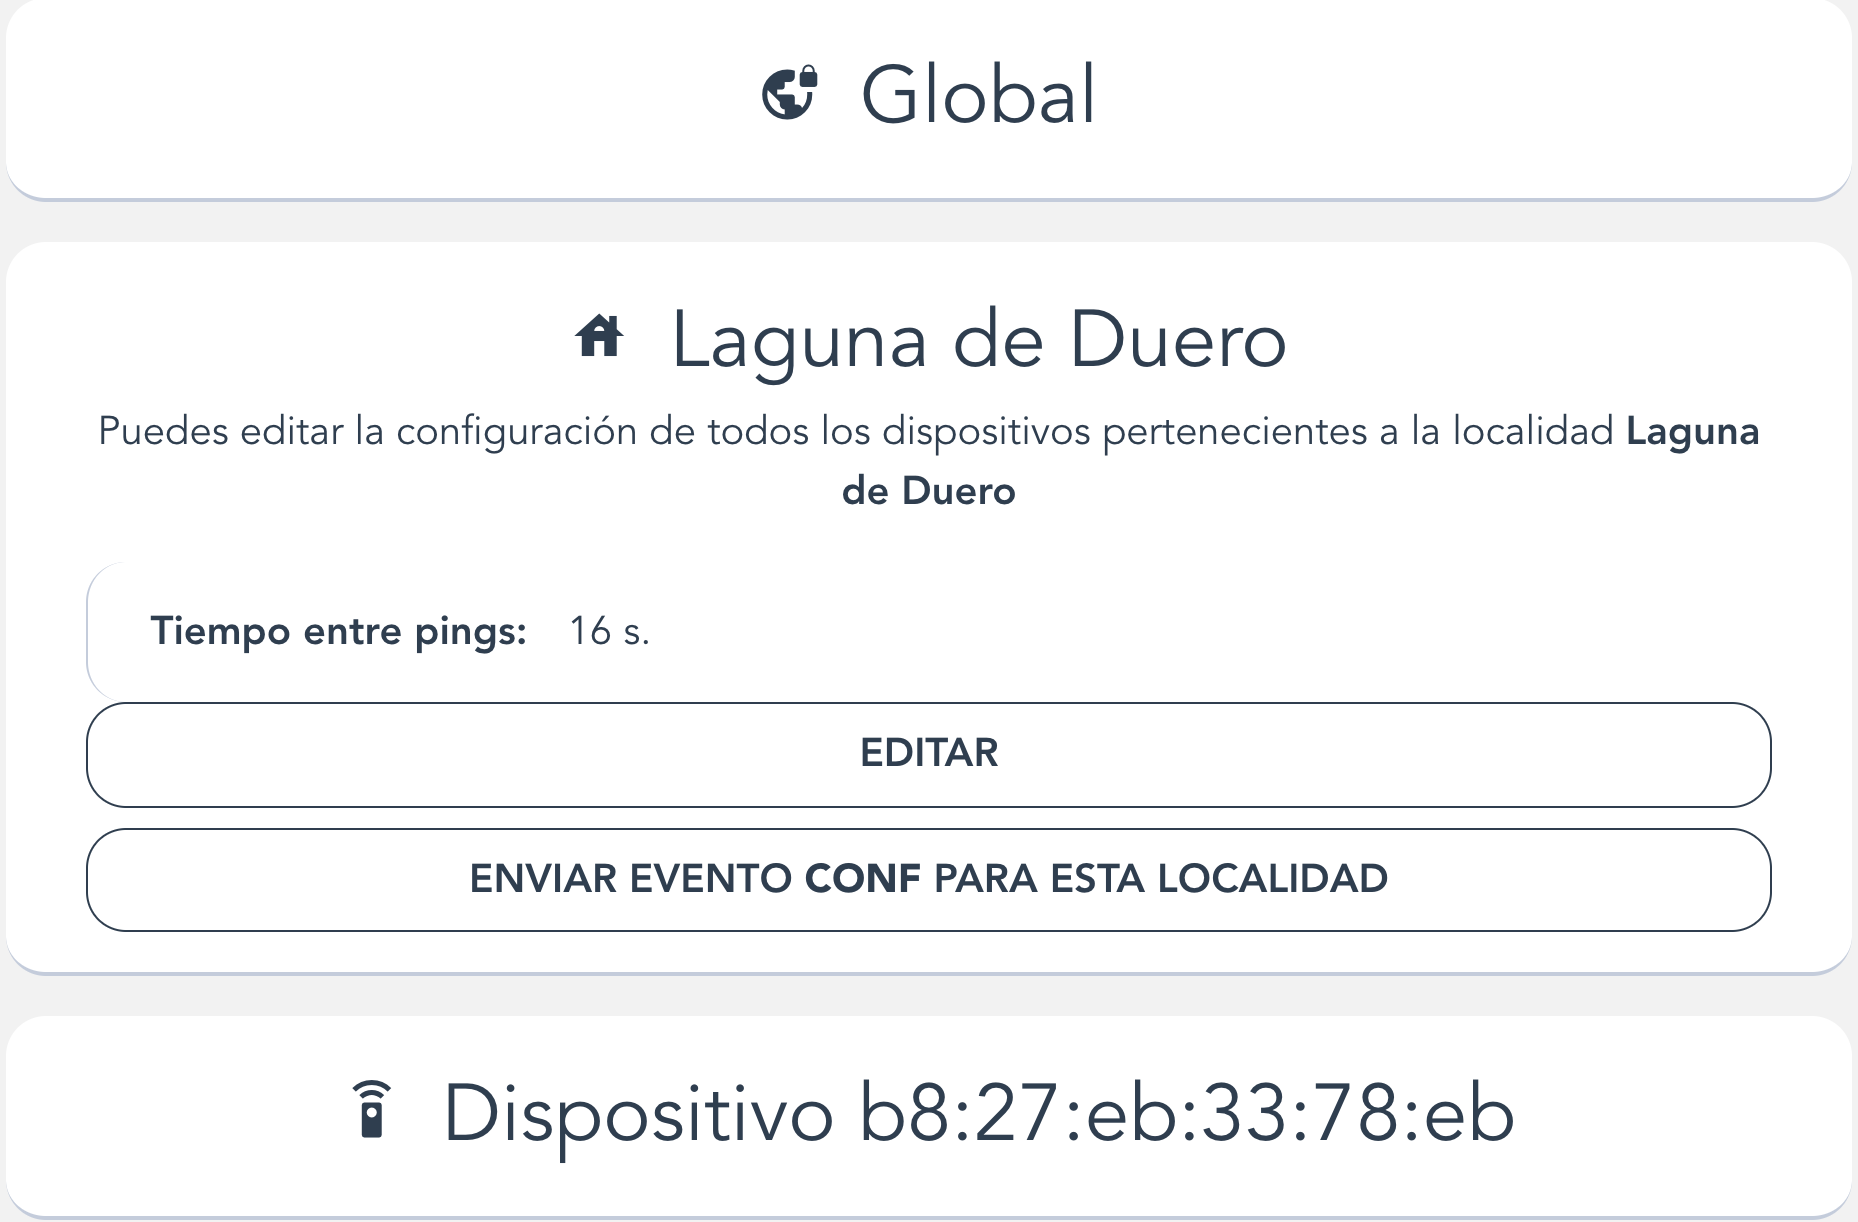
\includegraphics[width=10cm]{./img/web2/settings.location.png}
        \caption{Settings - Diseño final de configuración local.}
        \label{fig:set.local}
    \end{figure}
    
    \begin{figure}[H]   
        \centering
        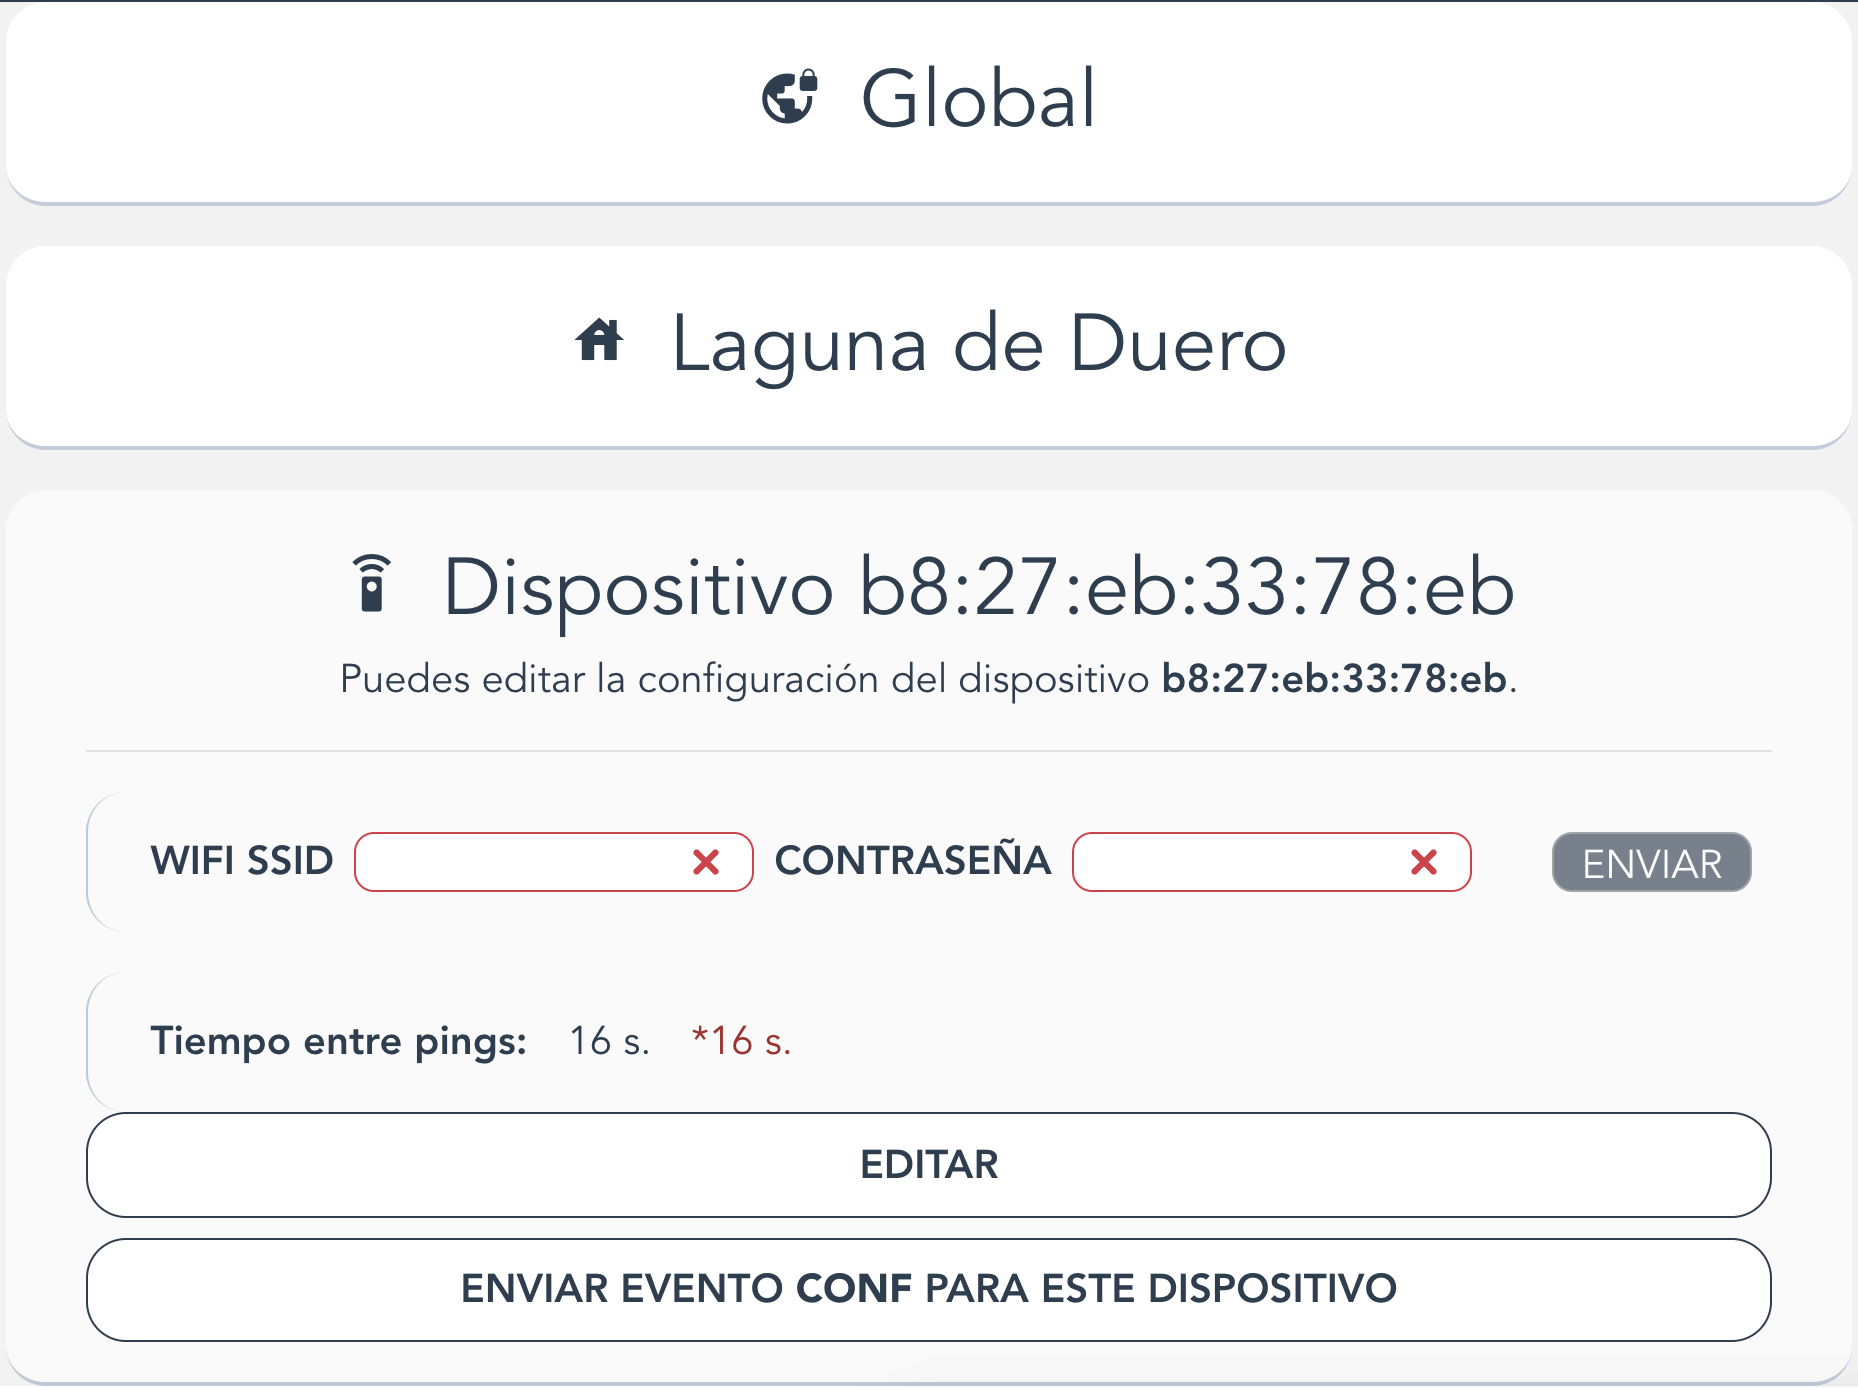
\includegraphics[width=10cm]{./img/web2/settings.device.png}
        \caption{Settings - Diseño final de configuración de un dispositivo.}
        \label{fig:set.device}
    \end{figure}
    
    
    \item \textbf{Usuarios} %%% USUARIOS
    
    Se mostrará una lista simple de todos los usuarios almacenados, de tal manera que aparezcan sus datos básicos, al igual que aparecerá su dispositivo asociado.
    La lista se debería poder filtrar en funcion del nombre, dni o dispositivo asociado con el fin de poder encontrar más fácilmente el usuario que se requiera.
    
    \begin{figure}[H]   
        \centering
        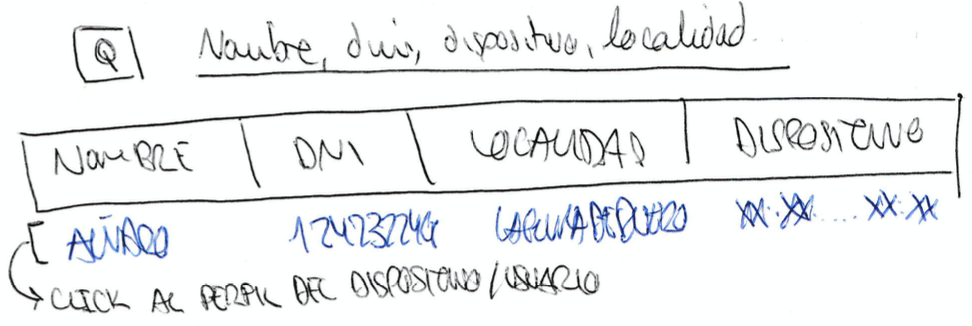
\includegraphics[width=10cm]{./img/web/users/users.pre.png}
        \caption{Users - Planteamiento de diseño de tabla de usuarios.}
        \label{fig:users.pre}
    \end{figure}
    
    \begin{figure}[H]   
        \centering
        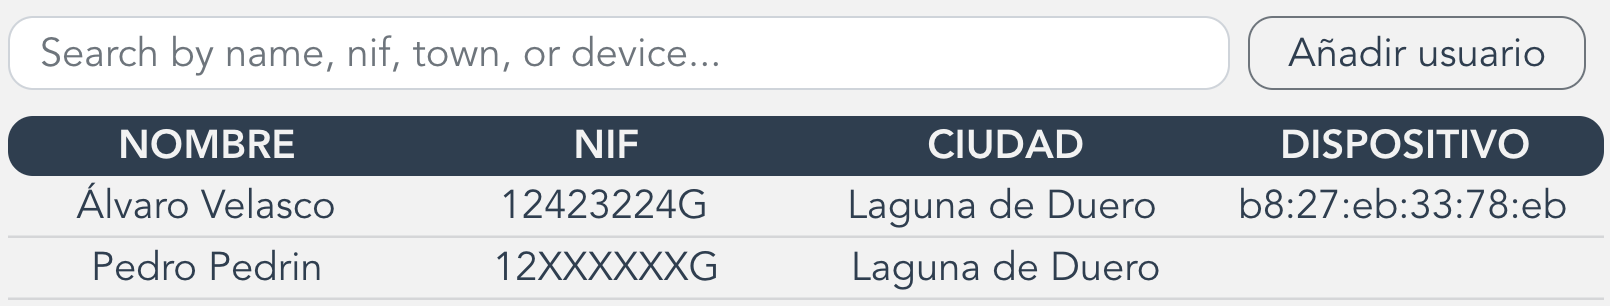
\includegraphics[width=11cm]{./img/web2/users.table.png}
        \caption{Users - Diseño final de tabla de usuarios.}
        \label{fig:users.post}
    \end{figure}
    
    También se debe dar la posibilidad de añadir usuarios nuevos al sistema, por lo que se realiza el diseño de un panel para añadir a los usuarios.
    
    \begin{figure}[H]   
        \centering
        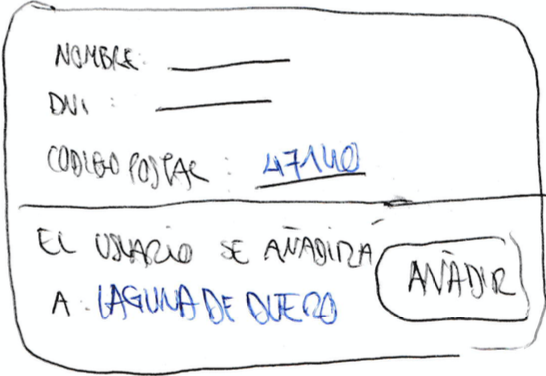
\includegraphics[width=6cm]{./img/web/users/users.add.pre.png}
        \caption{Users - Plantemiento de diseño de registro de usuarios}
        \label{fig:users.add.pre}
    \end{figure}
    
    A la hora de añadir usuarios, el código postal debe corresponder con el código postal de alguna ciudad ya registrada en el sistema, por lo que con tan solo ponerlo, ya te dice a qué localidad corresponde, si no, la aplicación web debería avisar sobre la necesidad de registrar anteriormente la localidad.
    
    \begin{figure}[H]   
        \centering
        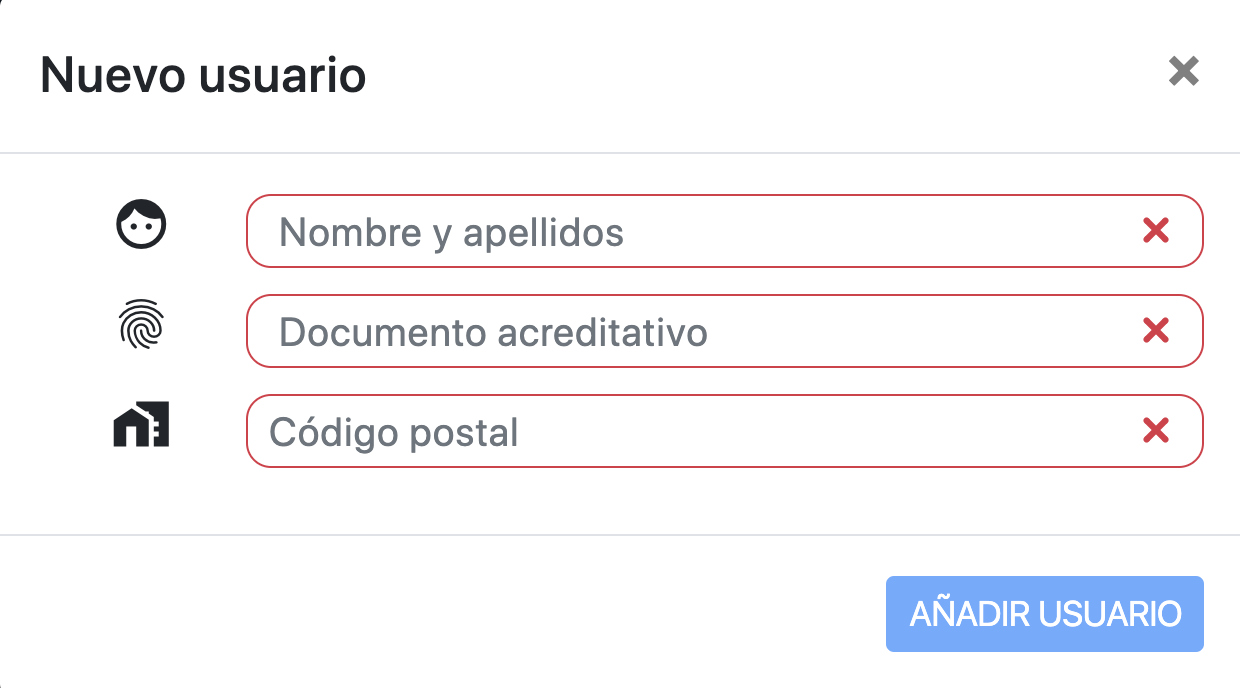
\includegraphics[width=10cm]{./img/web2/users.add.png}
        \caption{Users - Diseño final de registro de usuarios: código postal no registrado}
        \label{fig:users.add.fail}
    \end{figure}
        
    \begin{figure}[H]   
        \centering
        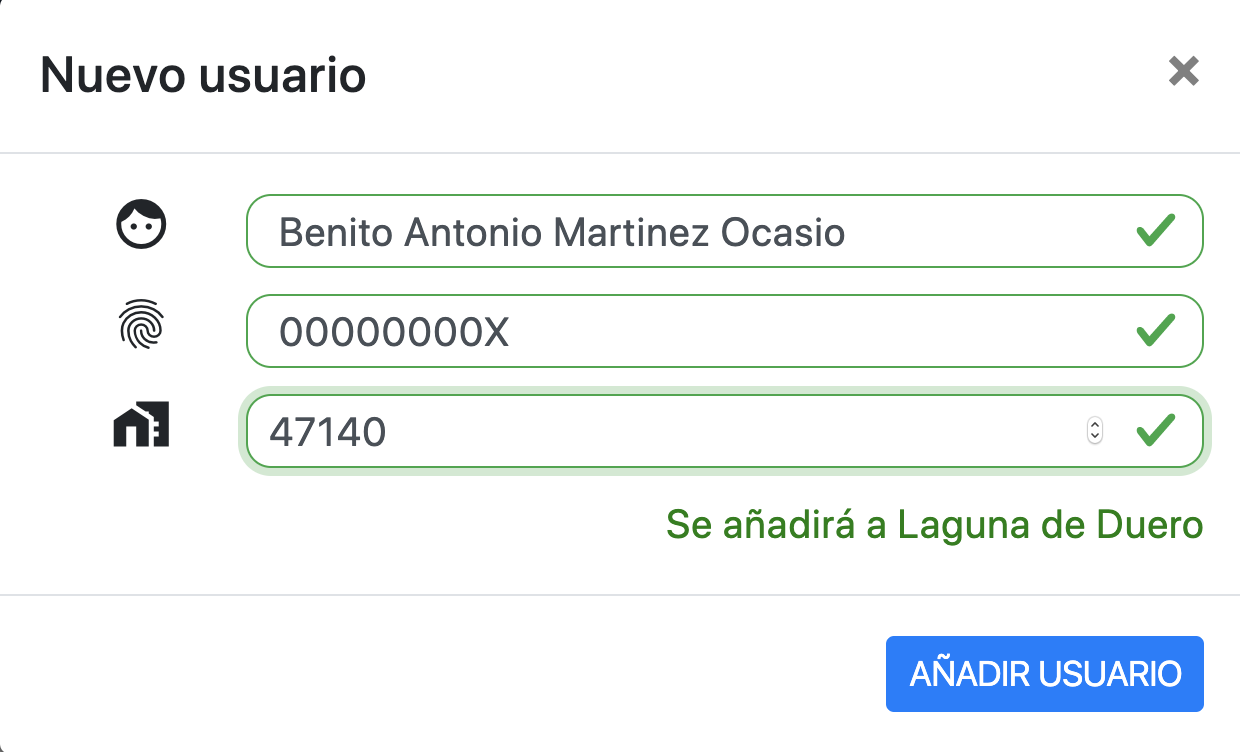
\includegraphics[width=10cm]{./img/web2/users.add.complete.png}
        \caption{Users - Diseño final de registro de usuarios}
        \label{fig:users.add.post}
    \end{figure}
        
    \item \textbf{Mapa} %%% USUARIOS
    
    La visualización a nivel estatal de la localización puede ser un buen aspecto para el control de los dispositivos, de modo que se pueda obsevar geográficamente cuántos dispositivos hay, y cómo están de dispersos por toda la geografía.
    
    Para ello se quiere poder mostrar un mapa donde aparezca un icono ubicado en la localización del usuario que lo tiene asignado, por lo que se necesita el diseño de ese icono:

    \begin{figure}[H]   
        \centering
        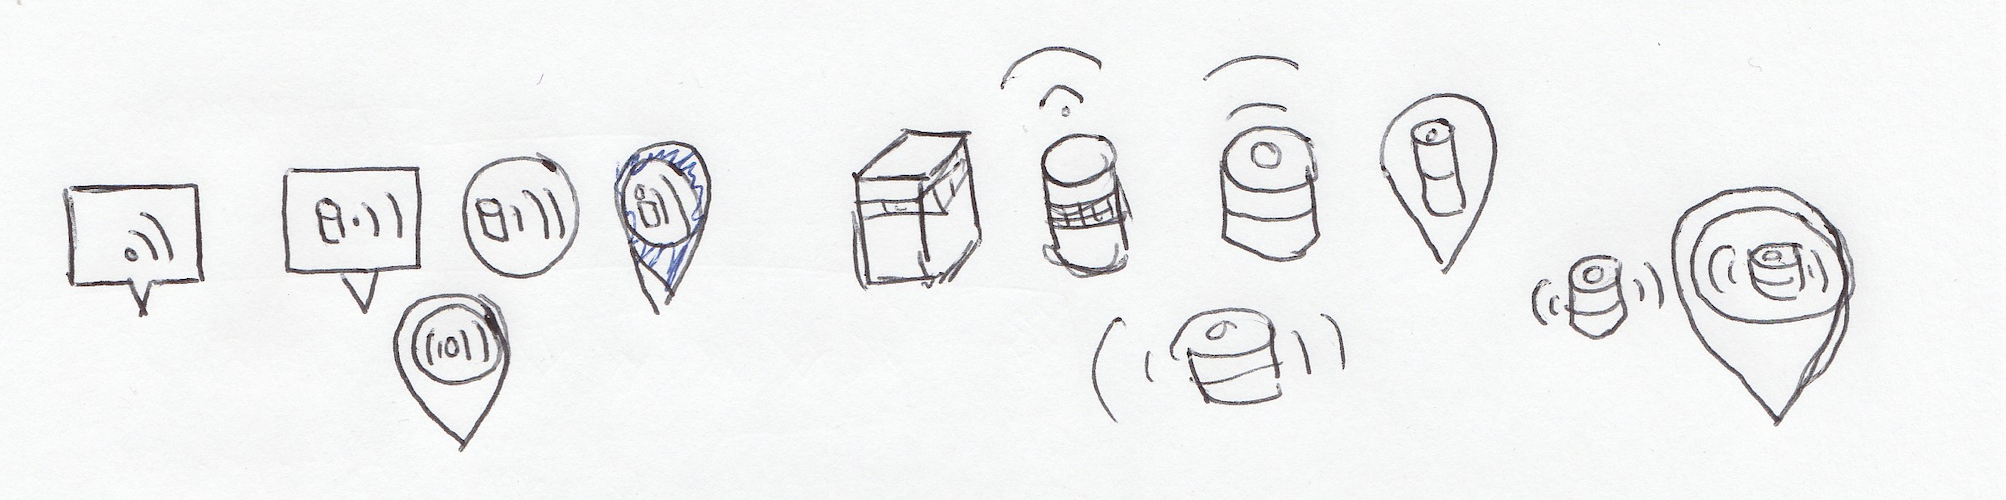
\includegraphics[width=13cm]{./img/icon/maps.icons.png}
        \caption{Mapa - Prototipo de iconos}
        \label{fig:icon.pre}
    \end{figure}

    El icono deberá aparecer en el mapa de color verde y ubicado en su lugar en caso de que el dispositivo esté asignado a algún usuario. En caso de que no tenga ninguna asignación, aparecerá en color amarillo, ubicado en la costa atlántica.
    
    \begin{figure}[H]   
        \centering
        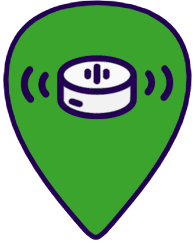
\includegraphics[width=3cm]{./img/icon/marker-green.png}
        \caption{Mapa - Marker de dispositivo asignado}
        \label{fig:icon.green}
    \end{figure}
    
    \begin{figure}[H]   
        \centering
        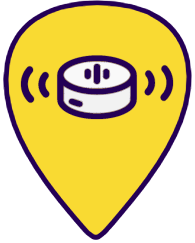
\includegraphics[width=3cm]{./img/icon/marker-yellow.png}
        \caption{Mapa - Marker de dispositivo no asignado}
        \label{fig:icon.yellow}
    \end{figure}
    
    \begin{figure}[H]   
        \centering
        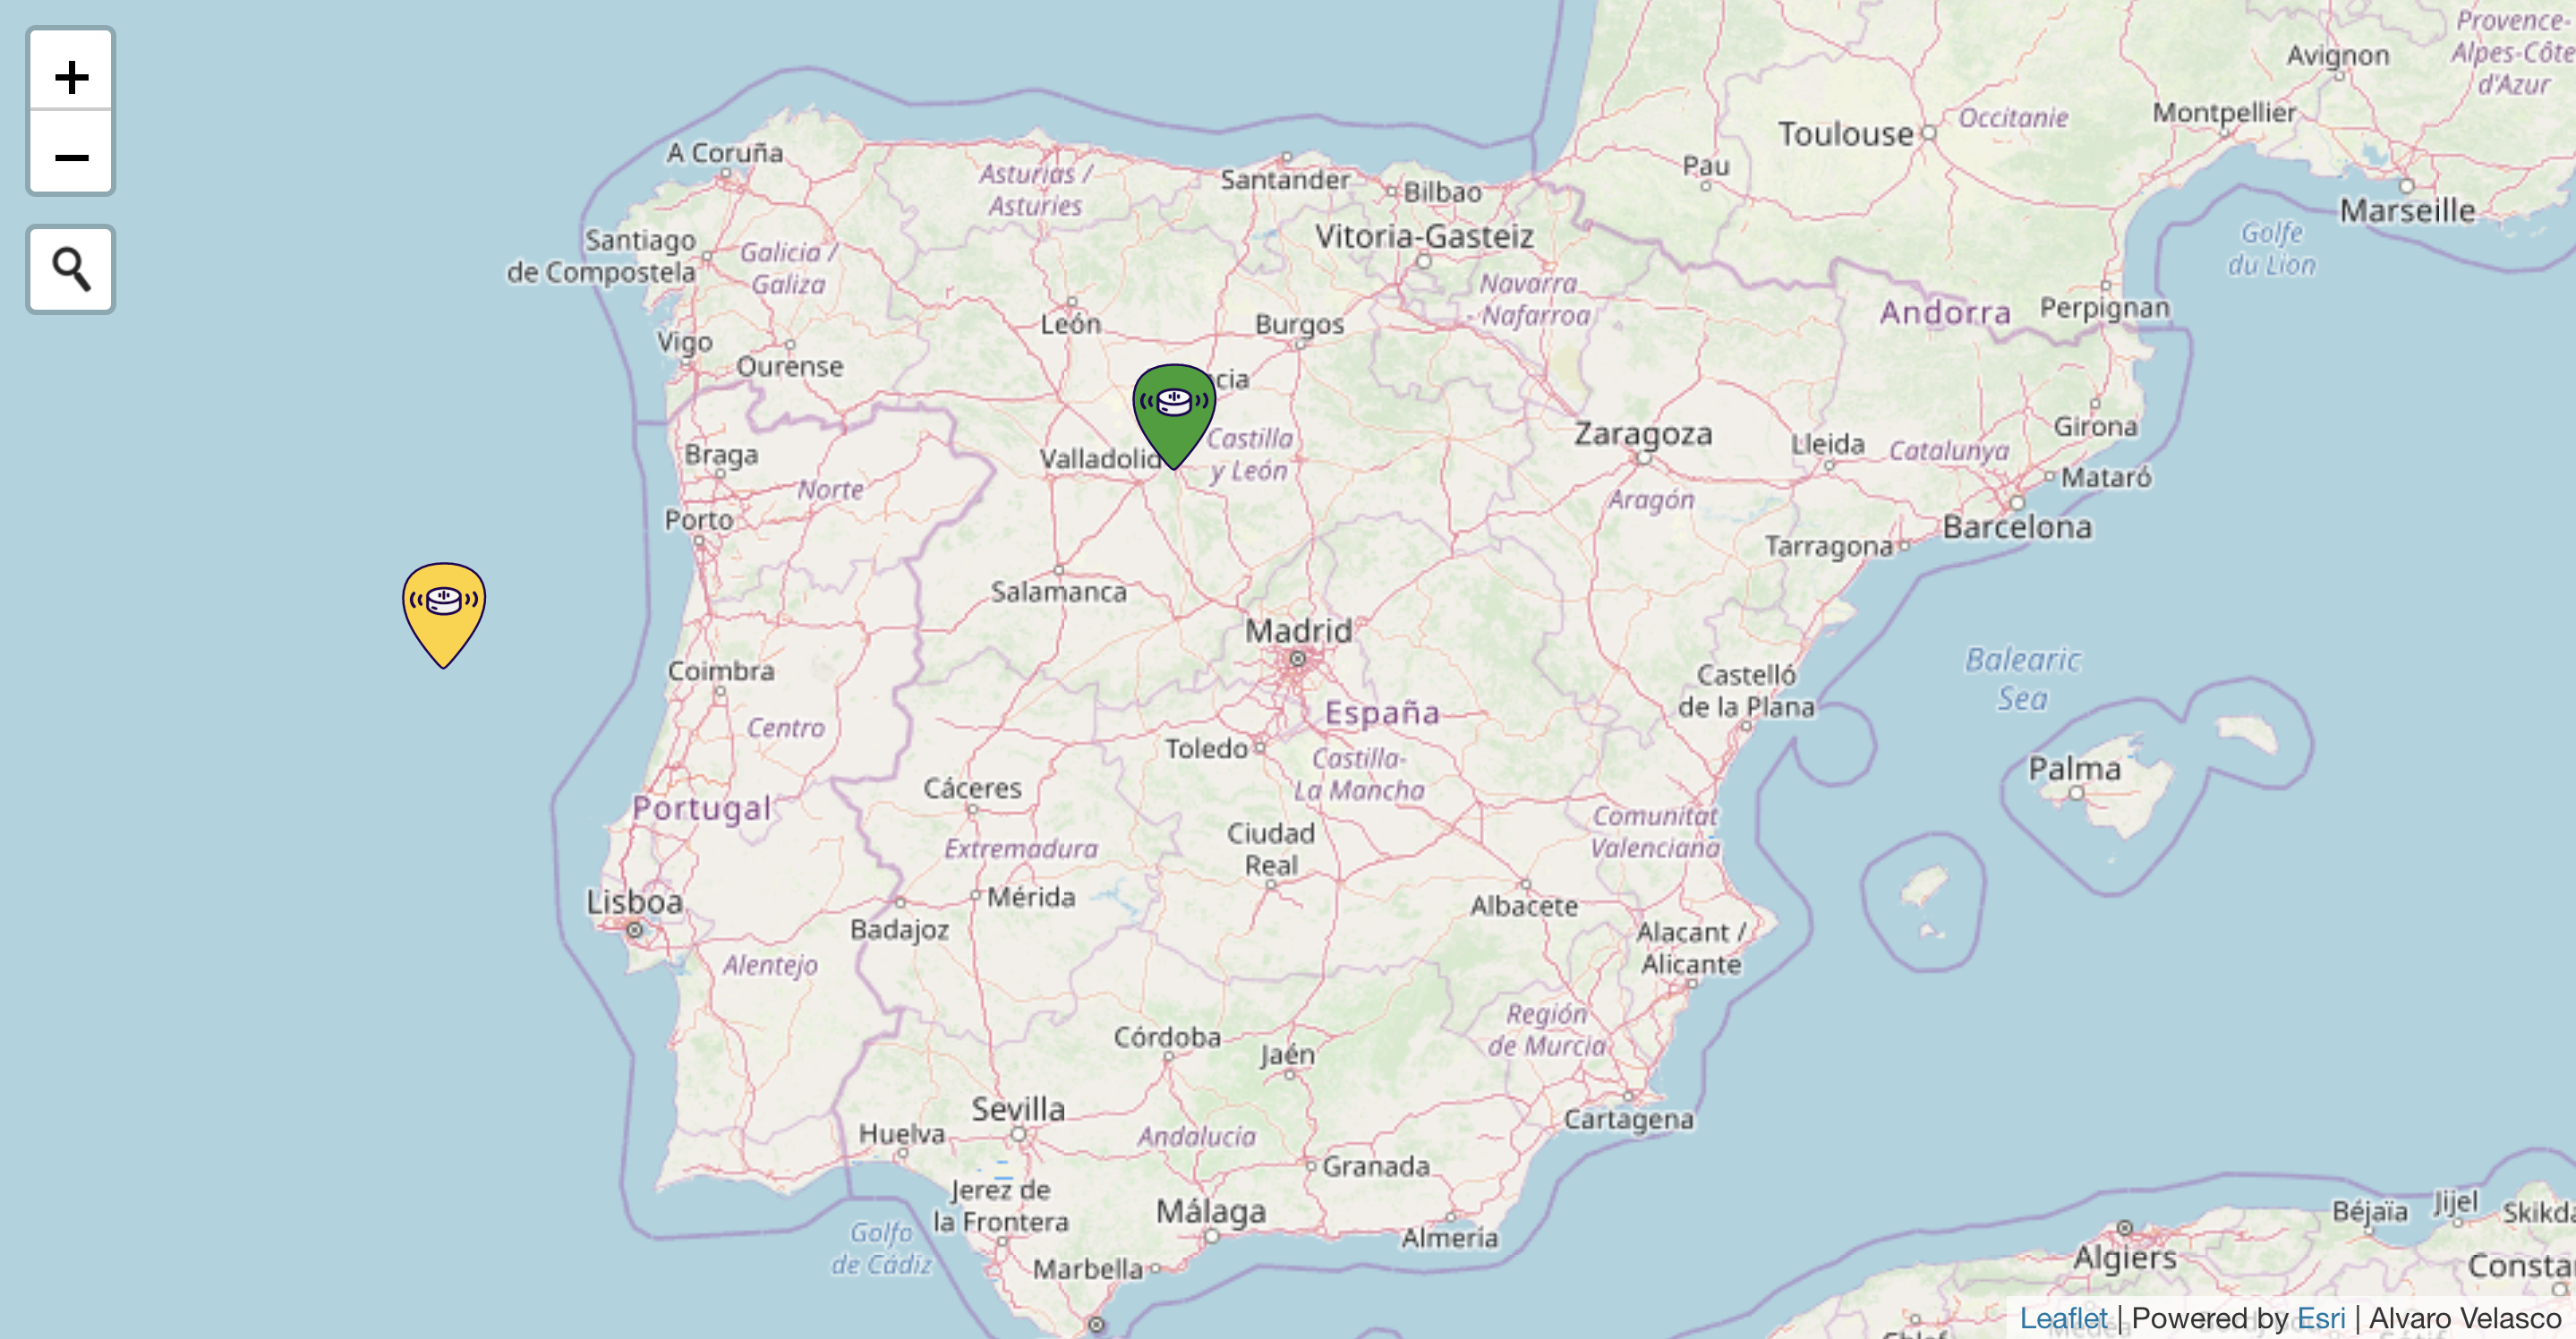
\includegraphics[width=11cm]{./img/web2/map.unassigned.png}
        \caption{Mapa - Diseño final: dispositivos separados}
        \label{fig:icon.yellow}
    \end{figure}
    
    En cuanto a los dispositivos mostrados en el mapa, se requiere que sean agrupados por localidades, mostrando el número en caso de que haya más de uno facilitando la representación y el número de ellos, como se ve en la figura \ref{fig:map.icon.grouped}, ya que mostrar todas las etiquetas juntas sería un problema de visualización. En caso de que se quiera conocer cuales son los dispositivos de la localidad, con tan solo dar click al número se acercaría el mapa y mostraría todos los markers sin solaparse, colocados en espiral y permitiendo, por tanto, la selección individual de cada uno de ellos.
    
        \begin{figure}[H]   
        \centering
        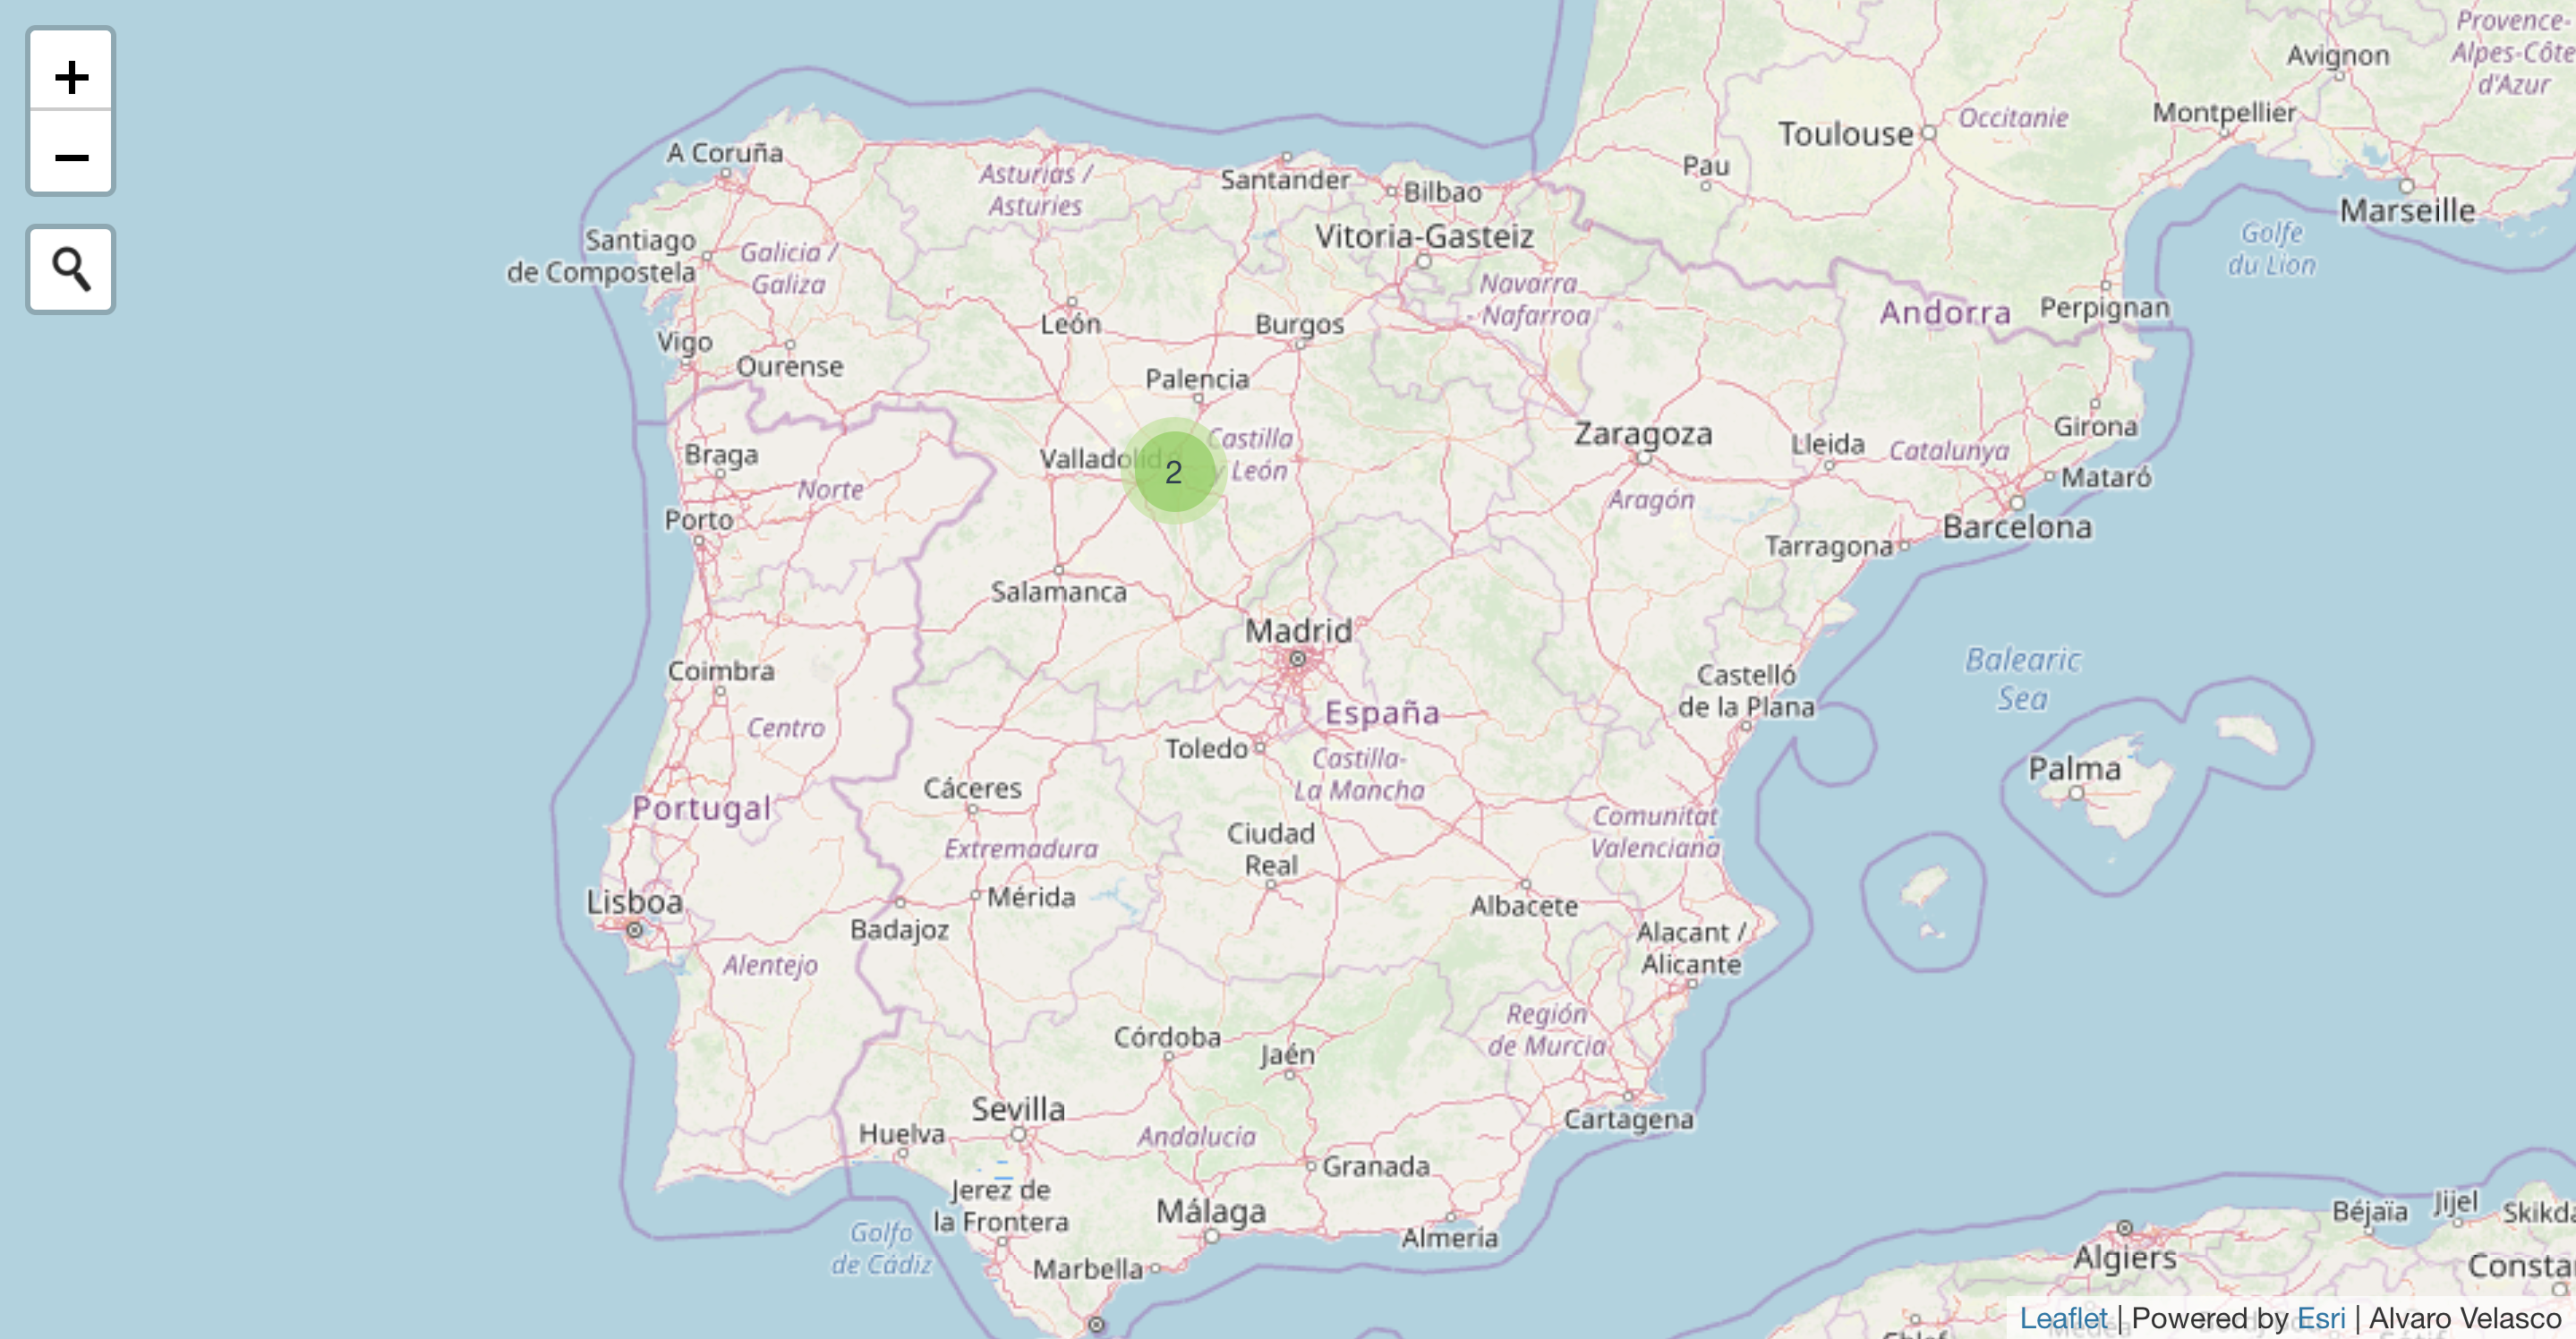
\includegraphics[width=11cm]{./img/web2/map.together.png}
        \caption{Mapa - Diseño final: agrupados por localidades}
        \label{fig:map.icon.grouped}
    \end{figure}
        
    \item \textbf{Perfil} %%% USUARIOS
    
    Las estadísiticas a mostrar en el perfil pueden ser tanto de un dispositivo sin asignar, como de un dispositivo asignado, como de un usuario sin dispositivo asignado.
    
    Debido a estas tres variantes se debe configurar la página de modo que permita ver ciertas funciones, ocultando otras, en función de qué es lo que se está observando.
    
    \begin{enumerate}
        
        \item Usuario sin dipositivo:
        Debe mostrar únicamente la información básica personal del usuario, y dar la posibilidad de asignar un dispositivo.
        
        \begin{figure}[H]   
            \centering
            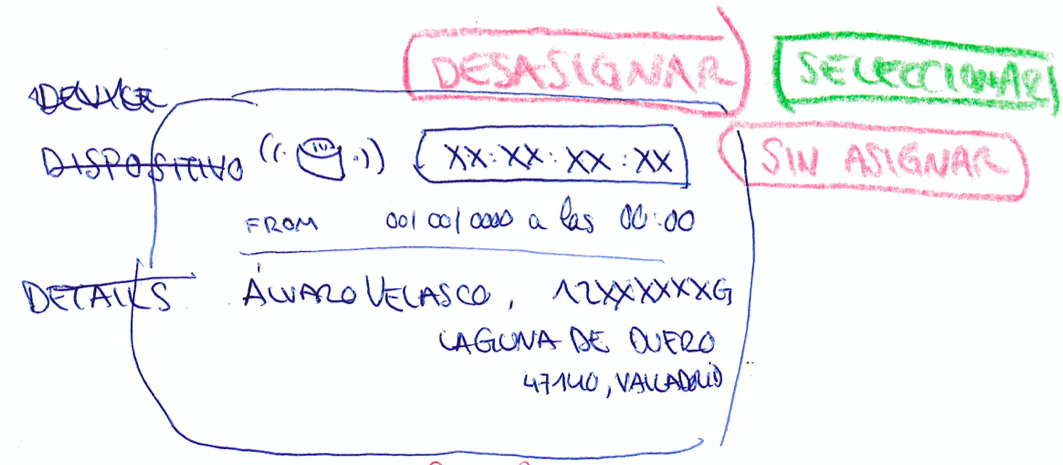
\includegraphics[width=8cm]{./img/web/perfil/stats.user.device.png}
            \caption{Perfil - Planteamiento de diseño de perfil de usuario/dispositivo}
            \label{fig:testfigura}
        \end{figure}
        El diseño final de esta variante puede verse en la figura \ref{fig:perfil.userlibre.post}.
        
        \item Dispositivo sin asignar:
        Debe permitir ver tanto las estadísticas globales de actividad, como las tareas realizadas, pendientes, y asignar nuevas tareas. Se hace un diseño previo sobre como debería mostrarse la tarjeta con la información del usuario, con la posibilidad de asignar o desasignar un dispositivo.
        
        \begin{figure}[H]   
            \centering
            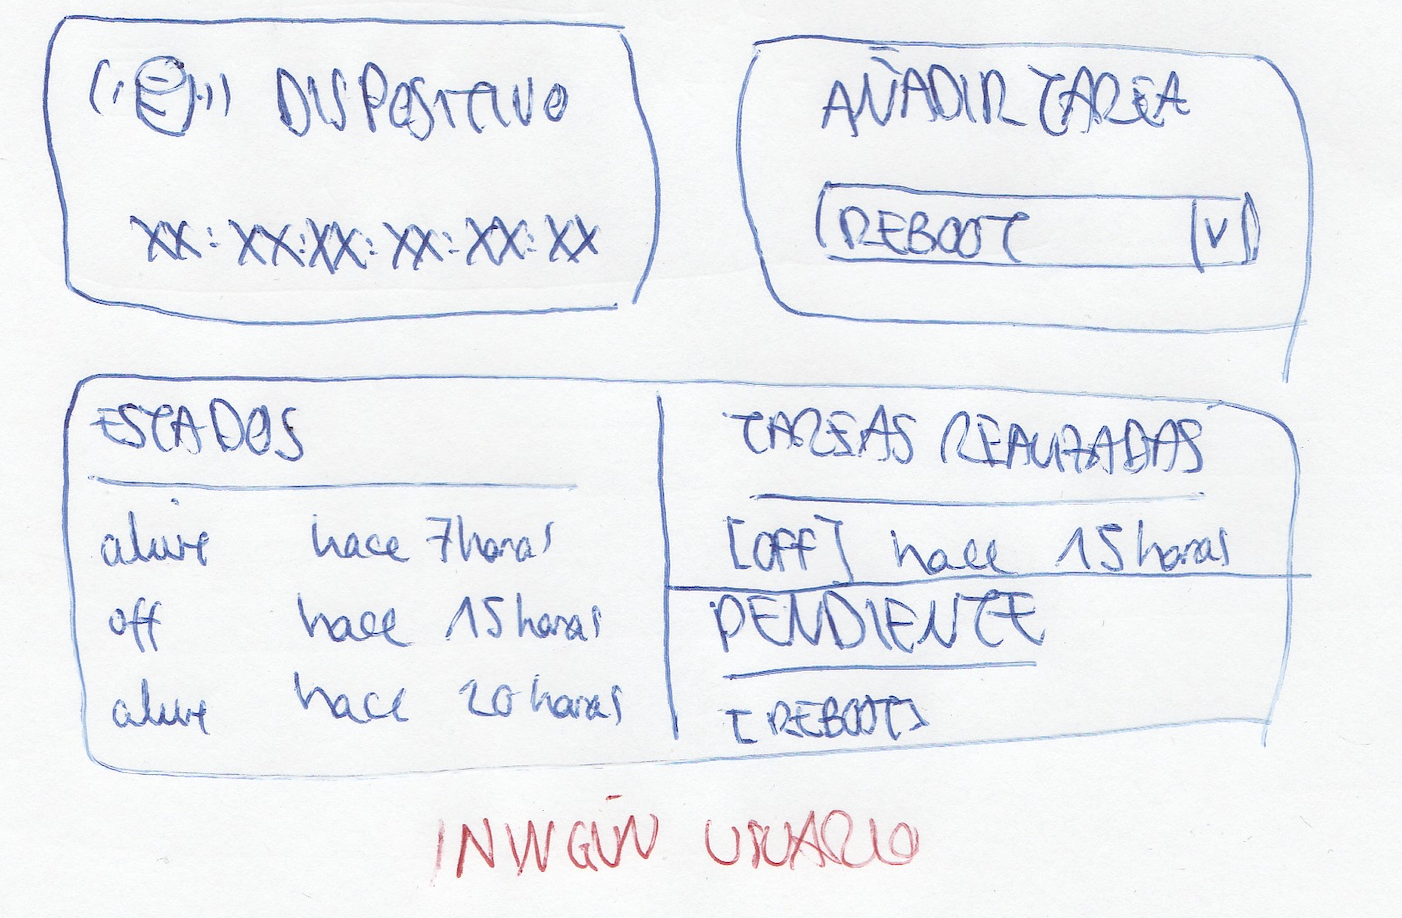
\includegraphics[width=8cm]{./img/web/perfil/stats.1.png}
            \caption{Perfil - Planteamiento de diseño de perfil de dispositivo sin usuario}
            \label{fig:perfil.tareas}
        \end{figure}
        
        \item Dispositivo asignado a usuario:
        Debe permitir ver tanto las opciones anteriores, limitadas por la fecha en que empezó la asignación, al igual que la información del usuario asociado, permitiendo desasignar al usuario el dispositivo, y asociar uno nuevo.
        
        \begin{figure}[H]   
            \centering
            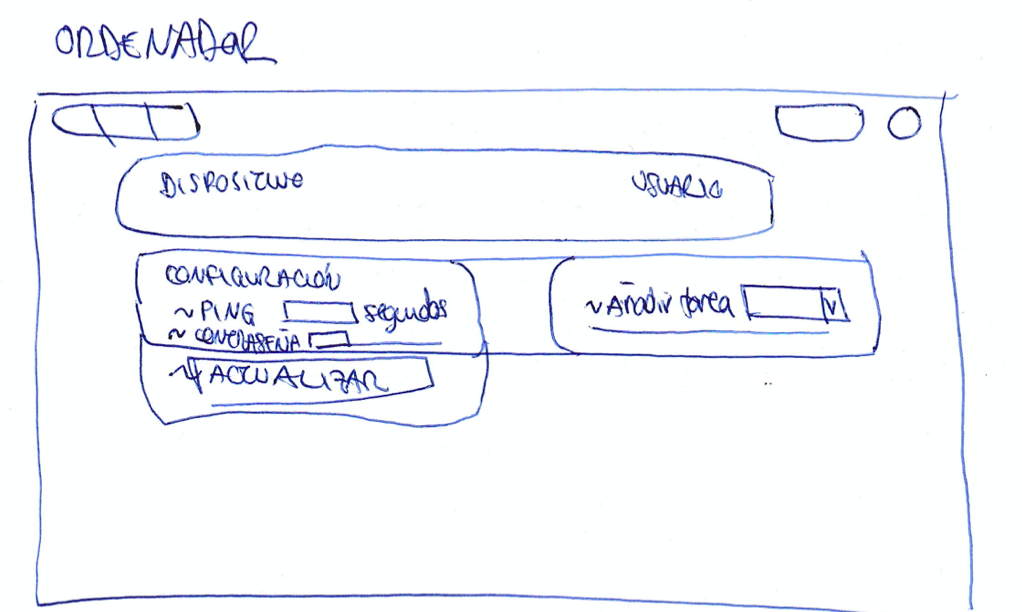
\includegraphics[width=7cm]{./img/web/perfil/device-all.pre.png}
            \caption{Perfil - Planteamiento de diseño de pagina}
            \label{fig:perfil.pag}
        \end{figure}
        
        En la figura \ref{fig:perfil.pag} se puede observar ya un diseño general de cómo será la vista de la página para todas las variantes, teniendo en cuenta las posibilidades que hemos nombrado anteriormente.
        En función del estado que se encuentre, se ocultaría el panel de usuario, o saldría la opción de asignar un nuevo dispositivo.
        También, este prediseño deja ver la colocación de todas las tarjetas, apareciendo la posibilidad de un diseño en el cual se pueda modificar la configuración o añadir tareas a realizar por el dispositivo, que solo estaría visible en caso de haberlo. 
        
        Una vez tratada la posibilidad de añadir tareas, la página debería facilitar la tarea de ver qué tareas se han realizado, o qué tareas hay pendientes, al igual que poder ver cómo ha interactuado el usuario con el dispositivo, o ver las estadísticas sobre cuál es la mayor cuestión con la que se interactúa con el dispositivo. Por ello, se plasta otra variante de diseño que permita todas estas funciones, como es representado en la figura \ref{fig:perfil.tareas2}
        
        \begin{figure}[H]   
            \centering
            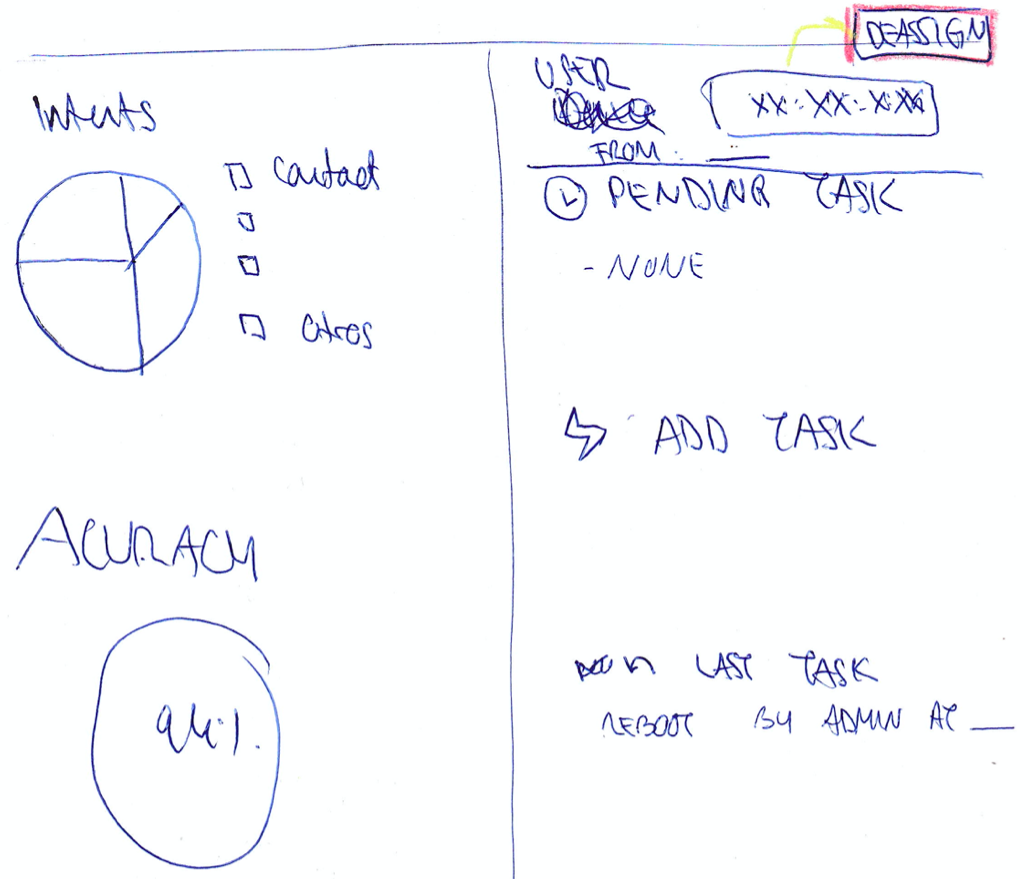
\includegraphics[width=7cm]{./img/web/perfil/stats.pre.png}
            \caption{Perfil - Planteamiento de diseño estadísticas}
            \label{fig:perfil.tareas2}
        \end{figure}
    \end{enumerate}
    
    Con este prediseño que da pie al muestreo de las estadísticas, una función útil sería el filtrado de ellas por fechas, pudiendo ser ese filtrado por días específicos, por meses, o por años.
    En cuanto a la posición de los filtros de las estadísiticas, se establecerá en la parte superior de la página, favoreciendo la intuición del administrador, mostrando su prototipo en la figura \ref{fig:perfil.filter}, que finalmente se ha implementado tal cual se diseñó, como muestra la figura \ref{fig:perfil.filter.post}.
    \begin{figure}[H]   
        \centering
        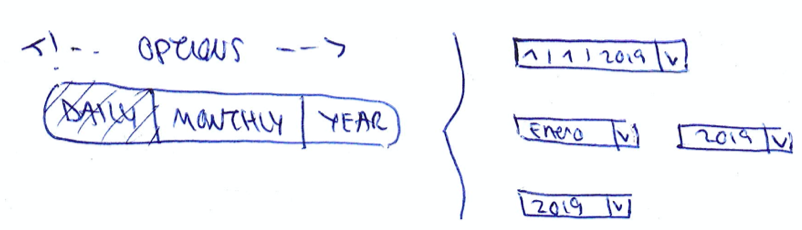
\includegraphics[width=8cm]{./img/web/perfil/stats.filter.png}
        \caption{Perfil - Planteamiento de diseño de filtro.}
        \label{fig:perfil.filter}
    \end{figure}
    
    \begin{figure}[H]   
        \centering
        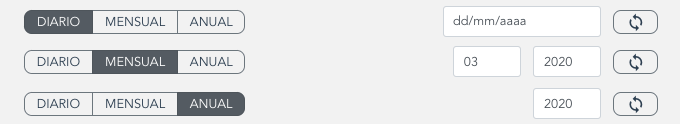
\includegraphics[width=12cm]{./img/web/perfil/filter.post.png}
        \caption{Perfil - Diseño final de filtro. (Posibilidades)}
        \label{fig:perfil.filter.post}
    \end{figure}
    
    Finalmente, debido a la gran variante de posibilidades y prediseños de la página, se ha optado por una conjunción de todos los prediseños, dando prioridad a mostrar las opciones por tarjetas que serán colocadas en orden de mayor a menor uso del administrador, facilitando el acceso a todas las funcionalidades posibles.
    
    \begin{figure}[H]   
        \centering
        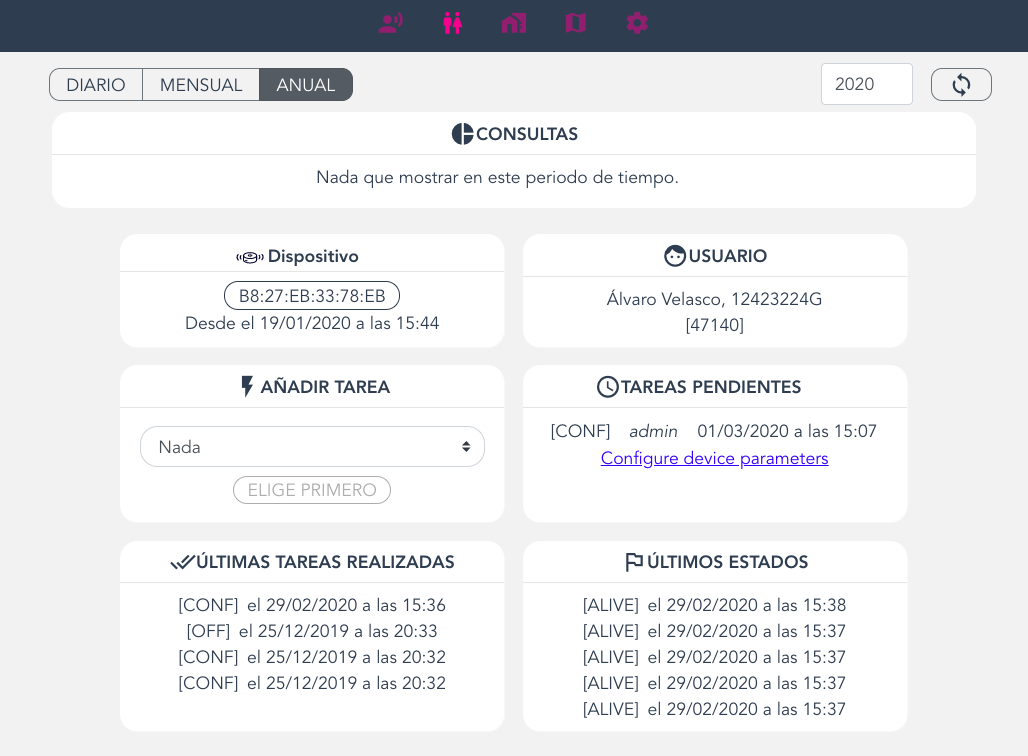
\includegraphics[width=12cm]{./img/web/perfil/stats.no-intents.png}
        \caption{Perfil - Diseño final del perfil: Usuario con dispositivo}
        \label{fig:perfil.dispositivoasignado.post}
    \end{figure}
    
    \begin{figure}[H]   
        \centering
        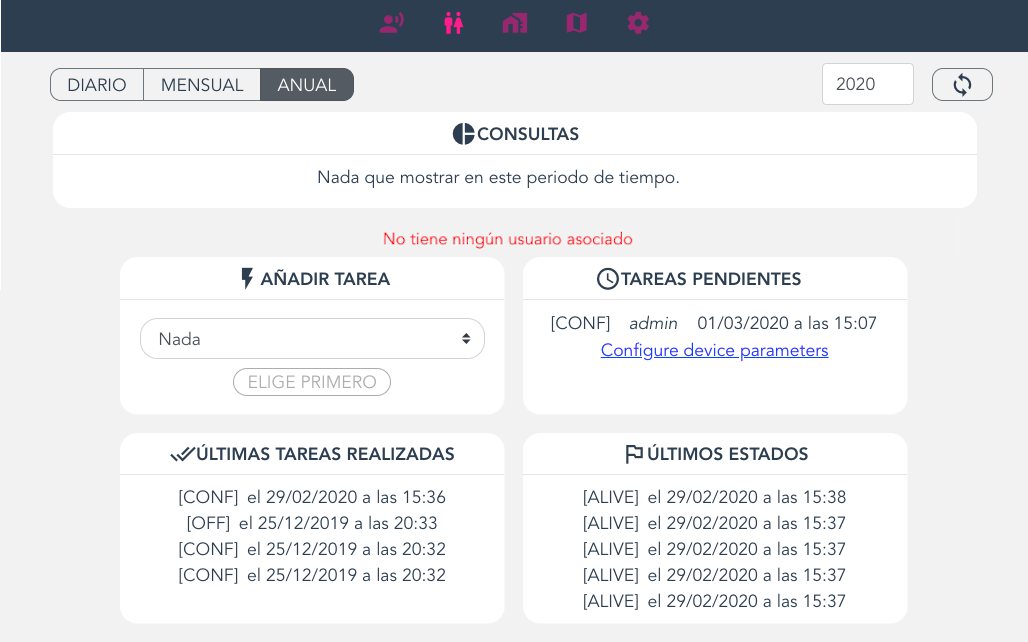
\includegraphics[width=12cm]{./img/web/perfil/stats.device.no-user.png}
        \caption{Perfil - Diseño final del perfil: Dispositivo libre}
        \label{fig:perfil.dispositivolibre.post}
    \end{figure}

    \begin{figure}[H]   
        \centering
        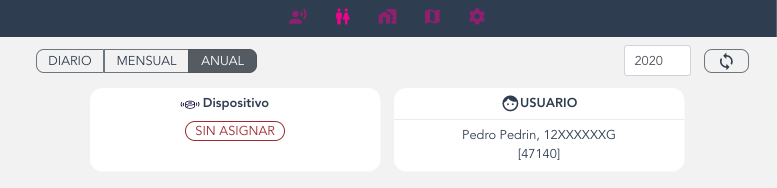
\includegraphics[width=12cm]{./img/web/perfil/stats.user.no-device.png}
        \caption{Perfil - Diseño final del perfil: Usuario libre}
        \label{fig:perfil.userlibre.post}
    \end{figure}
    
    Visto ya todo el sistema web, vemos que existe la posibilidad de asignar un dispositivo a un usuario específico, pero no se muestra como es esa asignación. Para ello, y pensando priorizar la usabilidad, se potencia mostrar una lista de los dispositivos que están disponibles, es decir, que no tienen ningún usuario asociado todavía. Esos dispositivos deberían estar apagados y amontonados en cajas en el despacho del administrador del proyecto. Por ello, y planteando lo que el administrador haría, sería conectar un dispositivo sin asignar, para ver que funciona. Por tanto, en la página, al mostrar los dispositivos sin asignar se ordenan poniendo los primeros los que han realizado un \textit{ping} de manera más reciente, ya que sería el que el administrador acabase de encender, como se muestra el prediseño en la figura \ref{fig:perfil.asign-device.pre}.
    
    \begin{figure}[H]   
        \centering
        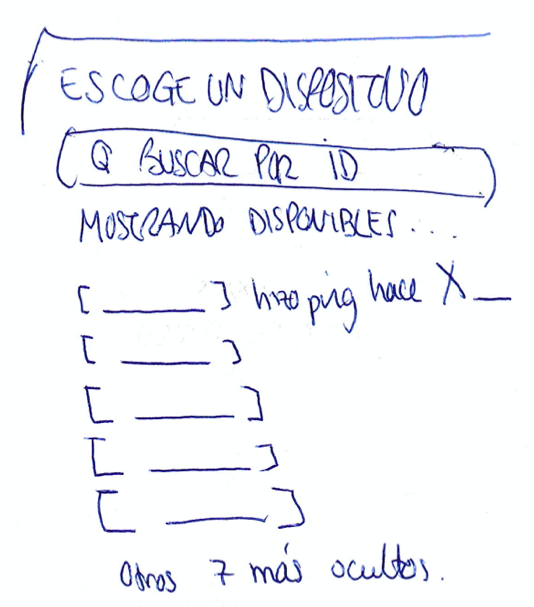
\includegraphics[width=5cm]{./img/web/perfil/stats.assign.png}
        \caption{Perfil - Pranteamiento de diseño de asignación de dispositivo}
        \label{fig:perfil.asign-device.pre}
    \end{figure}
    
    En el diseño final, mostrado en la figura \ref{fig:perfil.asign-device.post} no se realiza ningún cambio de diseño, dando por bueno y correcto el diseño previo.
    
    \begin{figure}[H]   
        \centering
        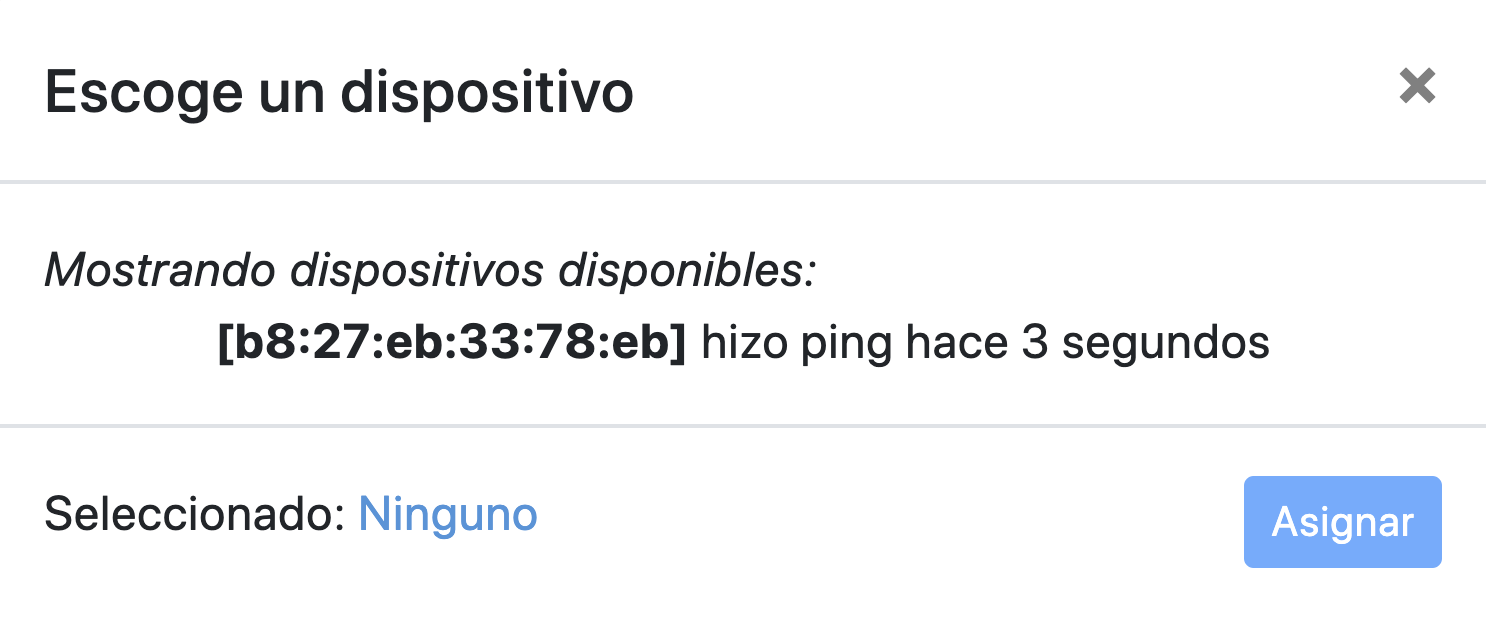
\includegraphics[width=9cm]{./img/web2/profile.add.device.png}
        \caption{Perfil - Diseño final de asignación de dispositivo}
        \label{fig:perfil.asign-device.post}
    \end{figure}
    
    En cuanto a las estadísticas sobre la actividad del usuario con el dispositivo, se ha optado por la opción de mostrar de base dos gráficas para las estadísticas:
    \begin{enumerate}
        \item Doughnut Chart: Para visualizar la relación entre la utilización de las distintas consultas.
        \item Gráfico de barras: Para visualizar a qué horas el dispositivo ha sido utilizado más veces. Esta gráfica puede ayudarnos en un futuro para ver en qué habitos del día a día se puede mejorar la experiencia del usuario.
    \end{enumerate}
    
    \begin{figure}[H]   
        \centering
        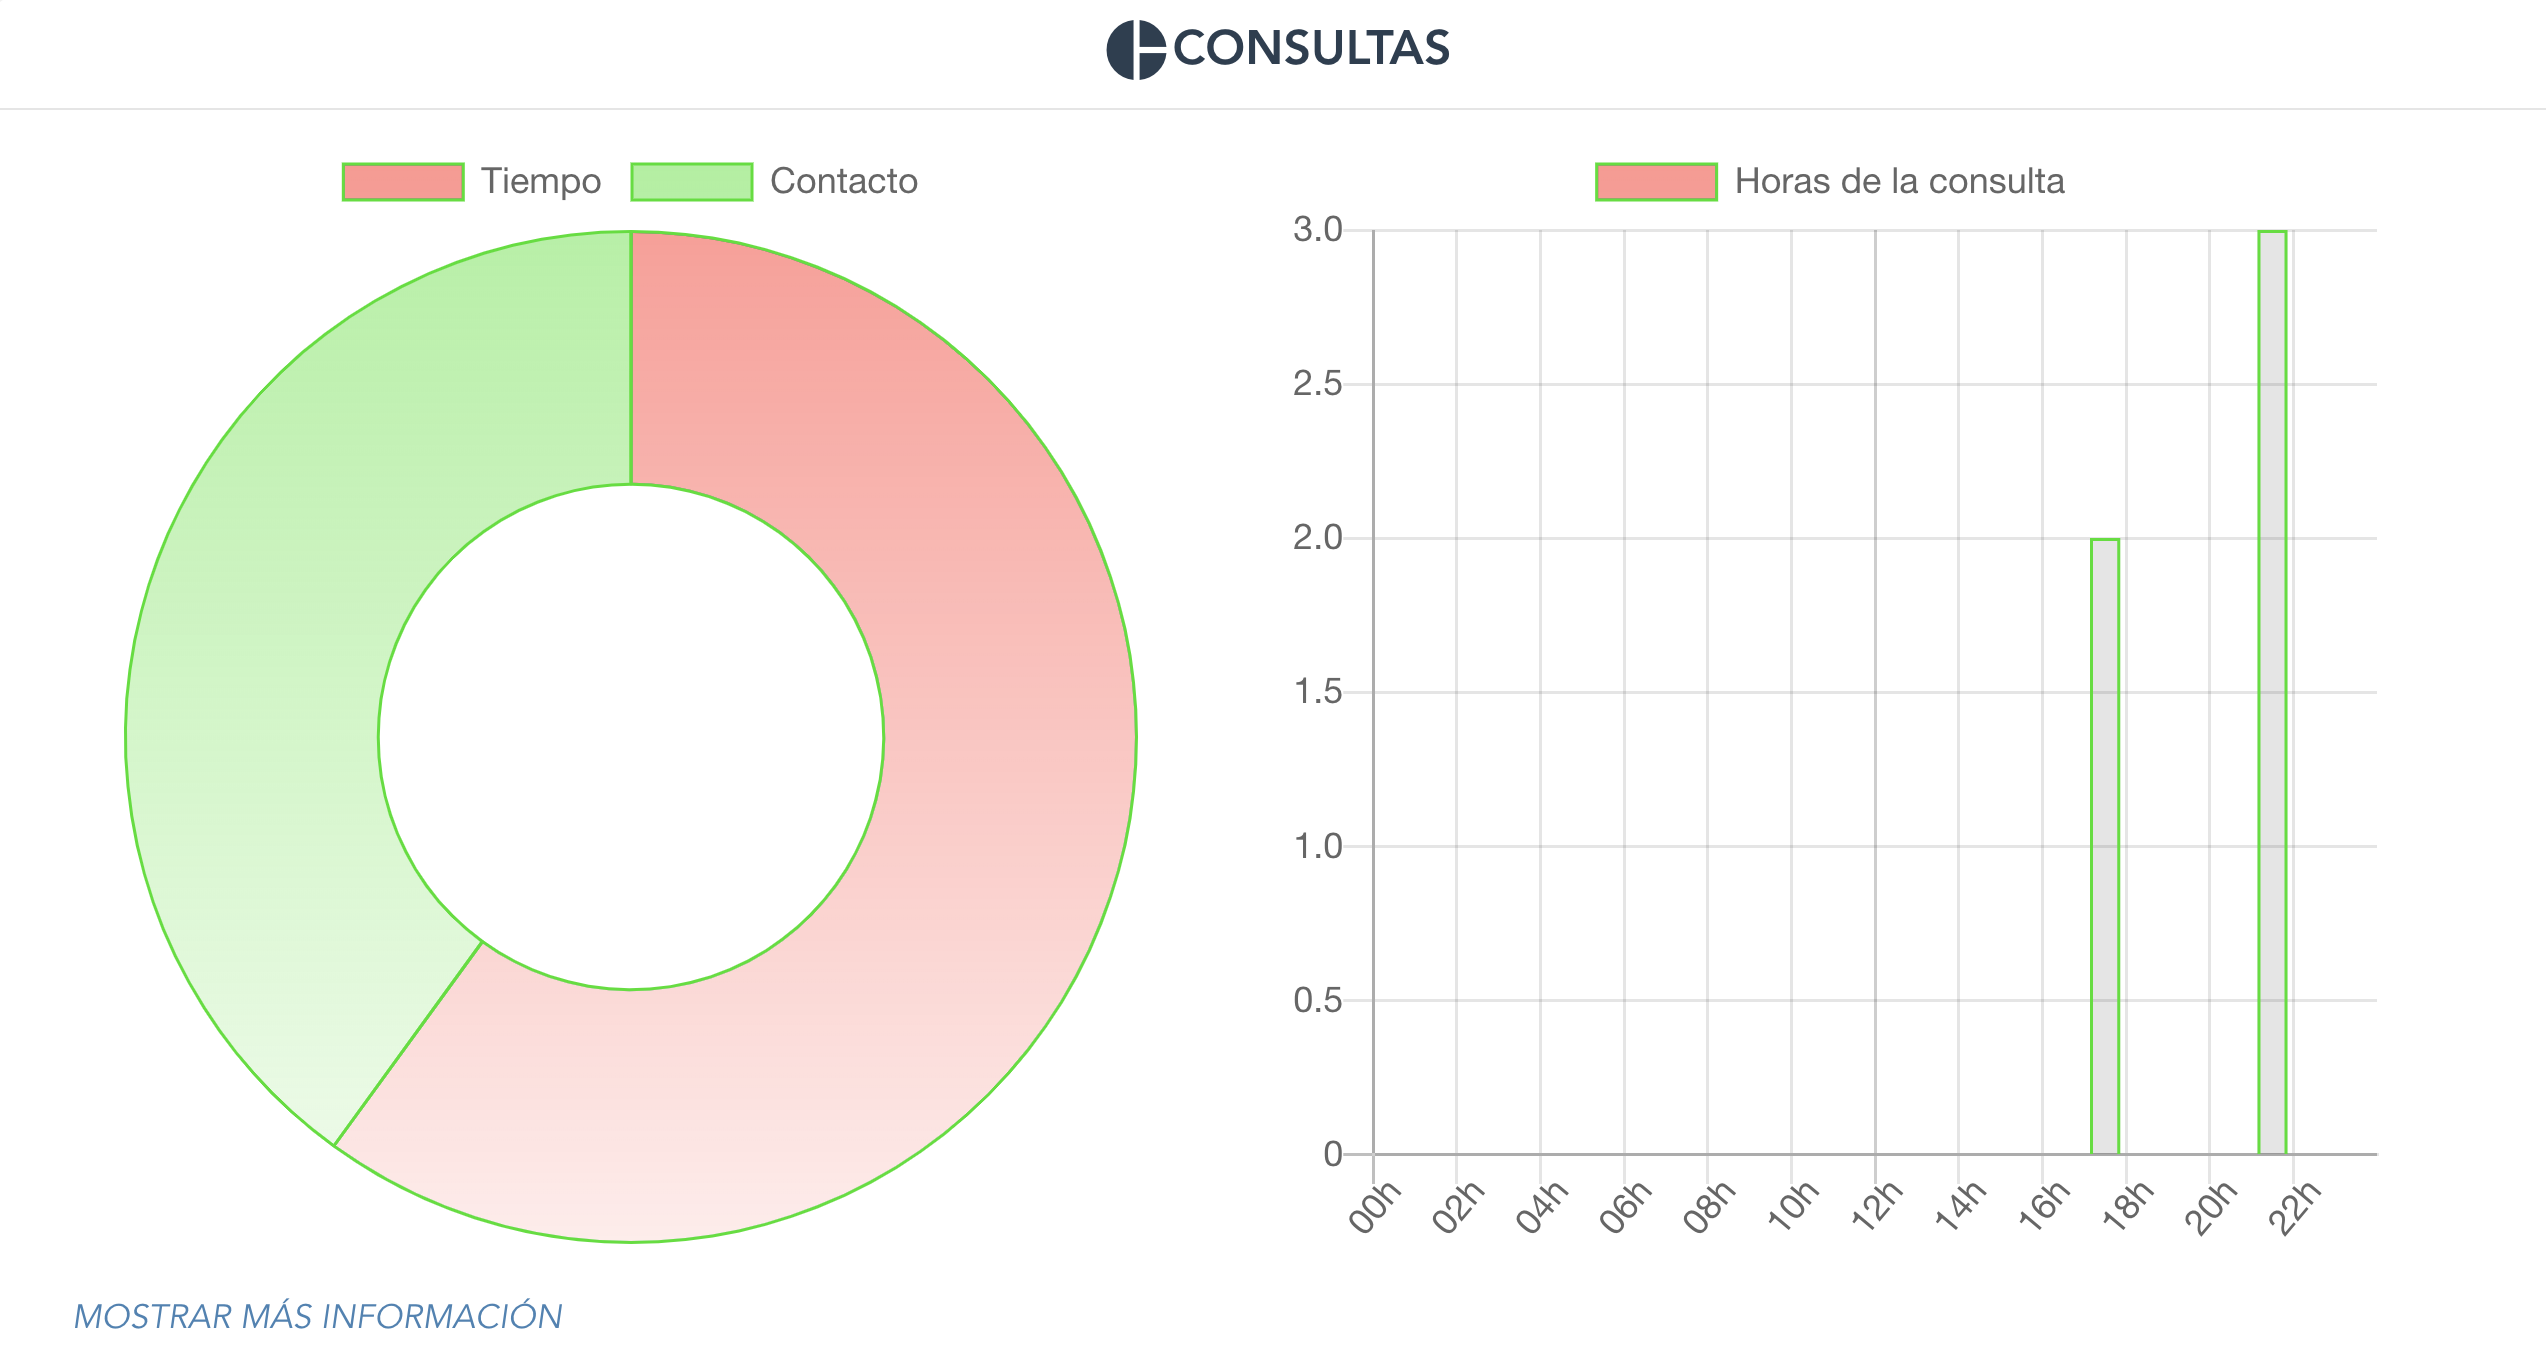
\includegraphics[width=12cm]{./img/web2/profile.stats.png}
        \caption{Perfil - Diseño final de consultas}
        \label{fig:perfil.consult.post}
    \end{figure}

    En caso de que se sospeche sobre un posible peligro acontecido en el hogar de nuestro usuario, se puede seleccionar la opción de \textit{Mostrar más información}, desplegando una tabla de color azul en la cuál aparecen las últimas 5 consultas que se han hecho al dispositivo, pudiendo identificar una consulta de auxilio, por ejemplo.
    
    Si se quiere más información sobre la información intercambiada en una consulta concreta se puede pulsar en la fila correspondiente, haciendo aparecer una segunda tabla en la cual se muestra la información relativa a esa consulta.
    
    \begin{figure}[H]   
        \centering
        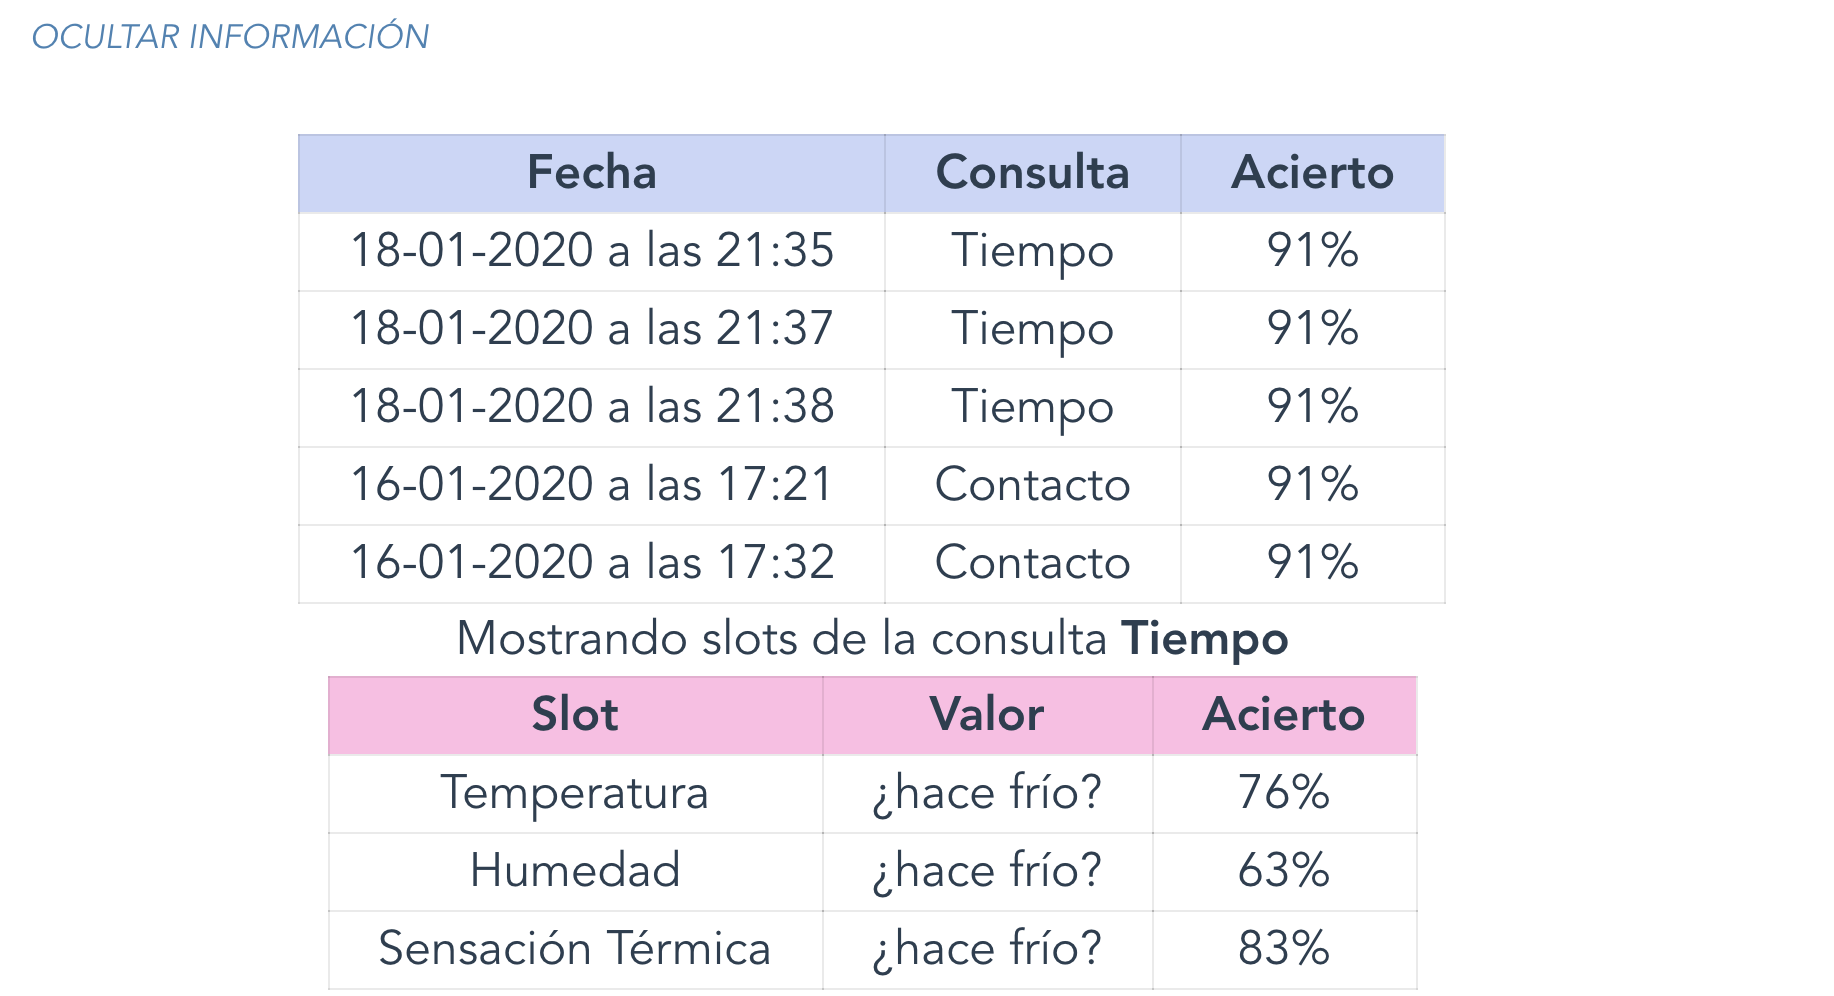
\includegraphics[width=12cm]{./img/web2/profile.stats.opened.png}
        \caption{Perfil - Diseño final consultas: Ampliado}
        \label{fig:perfil.consult.plus}
    \end{figure}
\end{enumerate}

    Como se puede observar en la figura \ref{fig:perfil.dispositivoasignado.post}, la vista, en caso de tener un dispositivo asignado, o ser una vista referida a la configuración de un dispositivo, que también se puede ver en la figura \ref{fig:perfil.dispositivolibre.post}, aparecen diferentes tarjetas, como de las últimas tareas realizadas que corresponde a las ordenadas por un administrador, o los últimos estados del dispositivo, donde se podrá ver si el dispositivo ha estado en uso, o simplemente está conectado \textit{(ALIVE)}, lo cual puede ayudar a la identificación de su uso de manera más rápida para el administrador.
    
    Otras tarjetas que se pueden ver son la de añadir una nueva tarea al dispositivo, donde se podría por ejemplo solicitar su actualización o apagado de manera remota. Una vez que se seleccionase una de estas tareas para realizarse, aparecerían en la tarjeta vecina, en la lista de tareas pendientes.
    
    Esta otra vista permite ver tanto las pendientes, como acceder a la configuración del dispositivo, que sería la figura \ref{fig:set.device}.